\chapter{初步认识计算机}

在真正学习计算机的有关内容之前,我们需要对计算机有一个最初步的认识。计算机是一个复杂的系统,它由许多不同的部件和组件组成,这些部件和组件共同工作以完成各种任务。

\section{计算机的发展历史}

人们一直在思考怎样进行更高效的计算。在古代,算盘、算筹等工具被用来进行计算。后来,随着科学技术的发展,人们对计算的需求越来越高,开始设计和制造更复杂的计算设备。查尔斯·巴贝奇(Charles Babbage)被认为是计算机的鼻祖,他在19世纪设计了第一台机械计算机——差分机和分析机。虽然他的设计在当时没有被完全实现,但他的思想为后来的计算机发展奠定了重要的基础。后来,也出现了一些其他的机械或电子计算设备,例如赫尔曼·霍列里斯(Herman Hollerith)发明的打孔卡机,该机器用于处理美国人口普查数据。

我们一般认为,阿兰·图灵(Alan Turing)是赋予现代计算机灵魂的人。他在1936年提出了“图灵机”的概念,图灵机是一个抽象的计算模型,能够模拟任何计算机的计算过程。自此,问题被分为两类:能用图灵机解决的(或者称作“图灵可计算的”)和不能用图灵机解决的;遇到前者,我们就可以掏出图灵机计算。图灵机的提出为现代计算机科学奠定了基础。

然而,图灵机更多的是一种抽象概念,真正把计算机变成现实的是冯·诺依曼。冯·诺依曼在1945年总结前人经验,提出并推广了“普林斯顿架构”。后来这个架构也被称作“冯·诺依曼架构”,也就是我们现在所说的计算机的基本结构。冯·诺依曼架构的核心思想是将程序和数据存储在同一块内存中,这样计算机就可以根据程序的指令来操作数据。冯·诺依曼架构是现代计算机的基础,目前几乎所有的计算机都遵循这一架构。

第一台真正意义上的\textbf{通用电子数字计算机}是ENIAC(Electronic Numerical Integrator and Computer),它于1946年由约翰·莫克利(John Mauchly)和约翰·普雷斯珀·埃克特(J. Presper Eckert)设计和建造。ENIAC使用了电子管作为主要的计算元件,计算速度可达每秒5000次加法运算。ENIAC的出现标志着电子计算机时代的到来——虽然它一开始是十进制的,实际上也并没有采用冯·诺依曼架构;直到1947年之后才被部分改造,引入了类似冯·诺依曼架构的设计。

随着技术的不断进步,计算机经历了多次重大变革。1950年代,晶体管的发明使得计算机变得更小、更快、更可靠、更节能。1960年代,集成电路(IC)的出现进一步推动了计算机的发展,使得计算机的性能大幅提升。1970年代,微处理器(SoC)的出现使得个人计算机成为可能。1980年代,图形用户界面(GUI)的引入使得计算机更加易于使用。1990年代,互联网的兴起使得计算机成为全球信息交流的重要工具,计算机也因为SoC真正得到广泛应用而开始走进千家万户。计算机的计算能力也早已今非昔比,如今一台家用计算机的计算能力已经达到每秒数十亿次浮点运算(GFLOPS),而高端服务器和超级计算机的计算能力更是达到了每秒数万亿次浮点运算(TFLOPS)甚至更高。

时至今日,计算机已经成为我们生活中不可或缺的一部分。无论是在工作、学习还是娱乐中,计算机都发挥着重要的作用。随着人工智能、大数据、云计算等新技术的不断涌现,计算机的未来发展充满了无限可能。

非常有趣的是,ENIAC的“生日”正是1946年2月14日,也就是情人节。或许这也象征着计算机与人类之间的深厚情感纽带。

\section{现代计算机的组成}

计算机的组成可以分为\textbf{硬件}和\textbf{软件}两大部分。硬件是指计算机的物理部件,如中央处理器(CPU)、内存、硬盘、显示器等;软件是指计算机上运行的程序和操作系统,如Windows、Linux、macOS等操作系统,以及Google Chrome、Microsoft VS Code、Tencent QQ等应用程序。

\subsection{计算机的硬件}

计算机的\textbf{硬件},也可以叫做\textbf{设备},可以简单分为两类:一类叫做\textbf{主机设备},是计算机用来进行计算等工作的设备;另一类叫做\textbf{外设设备}(也可以叫做\textbf{输入输出设备}),是计算机与外界进行信息交互的设备。通常说来,前者是藏在机箱里看不见的,后者是我们能够直接看见的。

一个计算机的主机设备如图\ref{fig:computer-hardware}所示。下面将会逐个介绍这些设备。
\begin{figure}[ht]
  \centering
  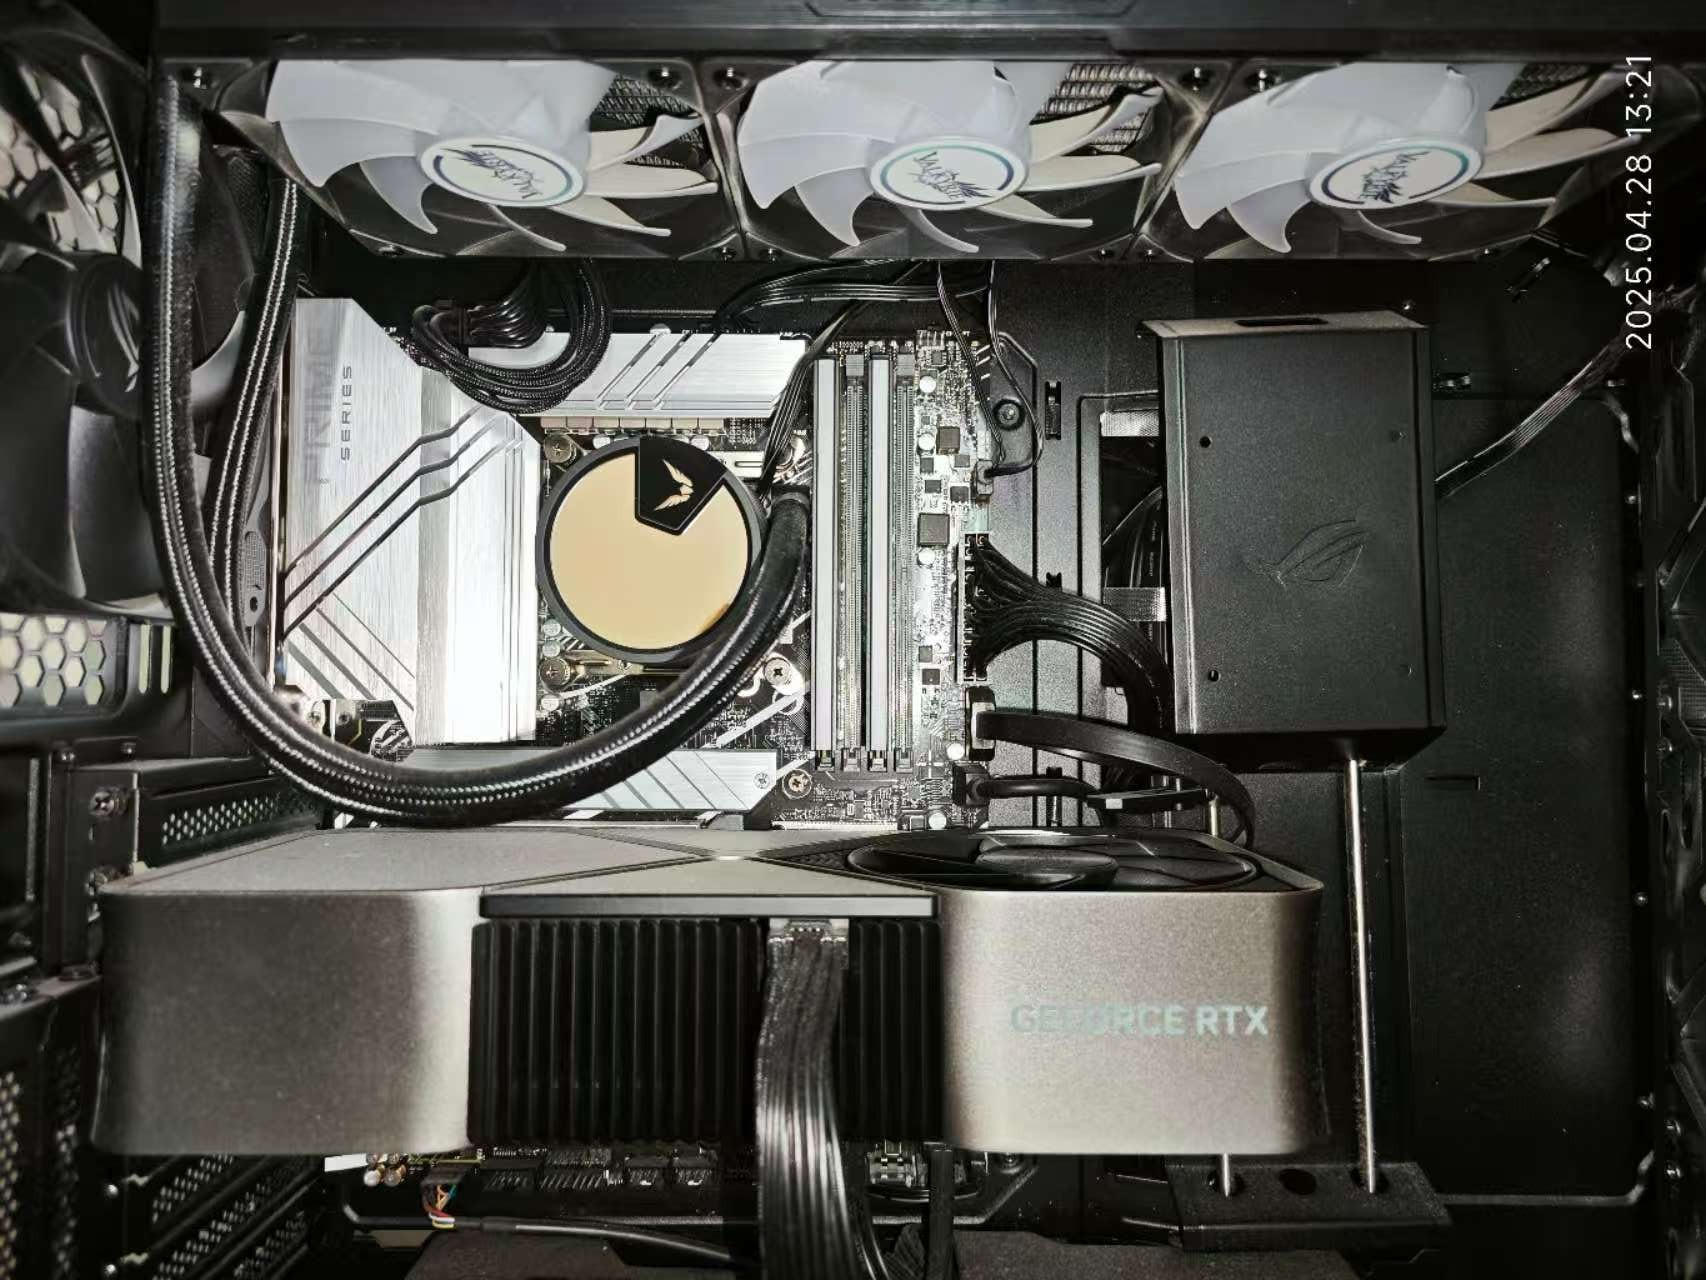
\includegraphics[width=0.8\textwidth]{100/hardware1.jpg}
  \caption{计算机的主机设备}
  \label{fig:computer-hardware}
\end{figure}

\subsubsection{中央处理器(CPU)}

CPU是计算机的最核心部件,它从存储设备读取指令和数据,并且执行这些指令。尽管现代处理器对代码和数据会有不同的处理,但是从程序员视角来看,其本质上都以二进制存储。代码由一条一条的指令组成,CPU 按照顺序一条一条执行从存储设备中读取的指令(至少从软件和程序员等使用者的视角看是这样),指令可以是修改 CPU 的状态,进行运算,或者是从其他硬件读取信息或者输出信息。如果希望进一步学习CPU如何运作等相关知识,可以参考著名的教材《CSAPP》,也可以修习《计算机系统导论》(ICS)这门课。

\subsubsection{内存(RAM)}

内存是计算机的临时存储器,它用于存储正在运行的程序和数据。它能够被CPU直接访问,因此速度较快。对于程序员而言,内存可以被抽象为一堆连续的存储单元,每个存储单元都有一个唯一的地址;执行程序时,程序的一部分或者全部被放进内存中,CPU就在内存中找寻需要的数据或者指令,如同在排列整齐的书架上寻找需要的书籍。

现代计算机内存读写速度很快,但是已经跟不上CPU的速度,因此又引入了高速缓存来加速内存的读写速度。高速缓存是内存和CPU之间的一个小型存储器,它存储了最近使用的数据和指令,以便CPU可以更快地访问它们。在断电以后,内存中存储的数据会丢失,因此内存也被称为是易失性的存储器。

\begin{note}
  上述文本中的“内存”指的是“随机存取存储器”(RAM)。这里的“随机”指的是可以在任意时刻访问任意地址,而不是“顺序存取”的存储器(例如磁带)。同时,“内存”这个词在部分语境下存在不同的含义,例如在BIOS语境下的“内存”指的是“只读存储器”(ROM),在移动设备(手机)等语境下的“内存”指的是“闪存”,这实际上是外存。
\end{note}

\subsubsection{外存}

外存是现代计算机的主要存储设备,用于存储操作系统、应用程序和数据等内容。其读写速度往往比内存慢得多,但是它的存储容量更大且往往是非易失的(相对内存而言)。

现代计算机的主要外存设备是硬盘。硬盘可以分为机械硬盘(HDD)和固态硬盘(SSD)。机械硬盘使用磁头在旋转的磁盘上读取和写入数据,而固态硬盘使用闪存芯片来存储数据。固态硬盘的读写速度比机械硬盘快得多,现在价格也便宜得多,但是使用寿命较短,且因为电荷流失等问题无法接受长期不通电等情况,不适宜作为长期存档介质(个人使用寿命和HDD无明显差异,基本都能用到彻底换机),除非花高价买高端的企业级SSD,但仍需定期通电。

除硬盘外,还有其他外部存储设备。例如:
\begin{itemize}
  \item U盘:一种小型的闪存存储设备,通常通过USB接口连接到计算机上。虽然和SSD都使用闪存颗粒,但是SSD通过主控优化、多通道技术等实现更高的性能,U盘则只用于低成本的便携存储。
  \item 光盘:一种使用激光读取和写入数据的存储介质。常见的光盘有CD、DVD和蓝光光盘,现在常用于单次写入的存档等。缺点是容易划伤和损坏,且信息密度低,读写速度慢。
  \item 磁带:一种使用磁性材料存储数据的介质,通常用于备份和存档。磁带的读写速度极为缓慢(和倒带速度成正比)且需要专门的设备来读写,设备价格昂贵,维护成本高。其优点是可靠性高,存储密度高。
  \item 软盘:一种老古董,使用磁性材料存储数据。现在软盘因为存储容量小、速度慢、易损坏等缺点,已经被淘汰了。
\end{itemize}

\begin{note}
  现代Windows系统的计算机中盘符默认从C开始而不是从A开始,正是因为AB盘符是给软驱用的;但是硬盘盘符从C开始的传统保留了下来,成为Windows的一个标志性特征。虽然现代的Windows系统允许手动分配盘符(如将C盘强行分配盘符A),但这样会导致系统不稳定,极不建议这么做。
\end{note}

\begin{caution}
\textbf{硬盘有价,数据无价。}请务必定期备份数据,尤其是重要数据。
\end{caution}

\subsubsection{显卡}

显卡是计算机的图形处理器,它用于处理图形和视频数据。显卡可以加速图形渲染,提高游戏和视频播放的性能。显卡通常有自己的内存,用于存储图形数据,被称为“显存”。

对于现在AI时代而言,显卡因为有着良好的并行特性,成为了通用深度学习的主流硬件之一。显卡的计算能力通常用“浮点运算每秒”(FLOPS)来衡量,通常情况下,显卡在机器学习等需要大量并行的简单计算工作上,表现远好于CPU。而在一些特殊的计算任务上,FPGA和ASIC等硬件则有着更好的表现,而部分嵌入式或边缘计算场景往往更偏好NPU或TPU等专用芯片。

\begin{tip}
  从上述例子中我们可以看到,CPU、GPU、TPU等的通用性是依次降低的,而在特定任务上的性能则是依次提升的。这种“专用性换取性能”的设计思路,是计算机体系结构中的一个重要原则,其一个重要体现就是软件硬件化,这也是近些年来兴起的“硬件加速器”设计思路的基础。
\end{tip}

\subsubsection{主板}

主板是一块电路板,将所有的硬件设备连接起来。主板上的芯片组负责协调各个硬件之间的通信。同时,主板还有一系列外部接口,用于连接外部设备。

\subsubsection{电源}

电源是计算机的电源供应器,它不参与数据存储与运算等操作,但能够为计算机的各个部件提供所需的稳定工作电压和电流。优质的电源能够避免计算机在运行过程中出现故障,延长计算机的寿命。

\subsubsection{输入输出设备}

输入输出设备指的是计算机与外界进行信息交互的设备。输入设备用于将用户的输入转换为计算机可以理解的格式,而输出设备则将计算机处理后的数据转换为用户可以理解的格式。

最古老的输入设备是拔插电缆,后来变成打孔纸带;现代常见的输入设备包括键盘、鼠标、扫描仪、麦克风等;现代常见的输出设备例如显示器、打印机、音响等。

\subsection{计算机的软件}

计算机的软件指的是计算机的程序和数据的集合。它可以分为系统软件和应用软件两大类。

\subsubsection{操作系统}

操作系统是计算机的核心软件,它负责管理计算机的硬件和软件资源。操作系统提供了一个用户界面,使用户可以与计算机进行交互。我们可以认为操作系统是连接现代软件和硬件的桥梁。目前,常见的操作系统有Windows、macOS、Linux等。

\textbf{Windows}\faWindows 是目前占有市场份额最大的操作系统。它由微软公司开发,广泛应用于个人计算机。Windows以其易用性和兼容性而闻名,广泛支持各种软件和硬件设备,但是缺点是在多数开发场景中的配置非常复杂,但是通过WSL2等工具也可以弥补一部分,且对于游戏开发等场景Windows仍是首选(主要是因为新游戏几乎都需要先适配Windows)。另一方面,Windows的安全性相对较低,容易受到病毒和恶意软件的攻击。

\textbf{macOS}\faApple 是苹果公司开发的操作系统,专门用于苹果的计算机产品。macOS以其优雅的界面和强大的功能而闻名,同时安全性相当高。缺点也很明显,macOS的硬件和软件生态系统相对封闭,且只能在苹果的硬件上运行,因此价格较高。

\textbf{Linux}\faLinux 是一个开源的操作系统,它是一个类UNIX操作系统。其学习曲线陡峭,至今在传统个人计算机市场的占有率仍然远低于Windows和macOS,但在服务器和嵌入式系统使用一直占据主导地位。Linux的开源特性使得它可以被自由修改和分发,因此有很多不同的Linux发行版,例如Ubuntu、Debian、Arch等。

几个系统的比较见下表:

\begin{table}[ht]
  \centering
  \begin{tabular}{c|ccc}
    \toprule
    操作系统 & Windows & macOS & Linux \\
    \midrule
    使用难度 & 简单 & 简单 & 较复杂 \\
    价格 & 收费 & 收费 & 免费 \\
    硬件兼容性 & 高 & 低 & 中高到极高 \\
    软件生态 & 丰富 & 不太丰富 & 丰富 \\
    安全性 & 较低 & 高 & 高 \\
    系统级可定制性 & 较低 & 较低 & 高 \\
    社区支持 & 强 & 一般 & 强 \\
    适用场景 & 办公、游戏 & 设计、开发 & 服务器、开发 \\
    \bottomrule
  \end{tabular}
\end{table}

对于计算机新手,我们推荐使用Windows和macOS系统作为操作系统,这是因为它们提供了友好的用户界面和丰富的软件支持,适合初学者使用。对于希望深入学习计算机的初学同学,我们推荐使用Linux系统的发行版Ubuntu,因为它具有和Windows与macOS类似的图形界面,并具有良好的社区支持和丰富的学习资源。对于希望进阶的同学,我们推荐使用Arch Linux,它是一个轻量级的Linux发行版,具有高度的可定制性和灵活性。

\begin{figure}[ht]
  \centering
  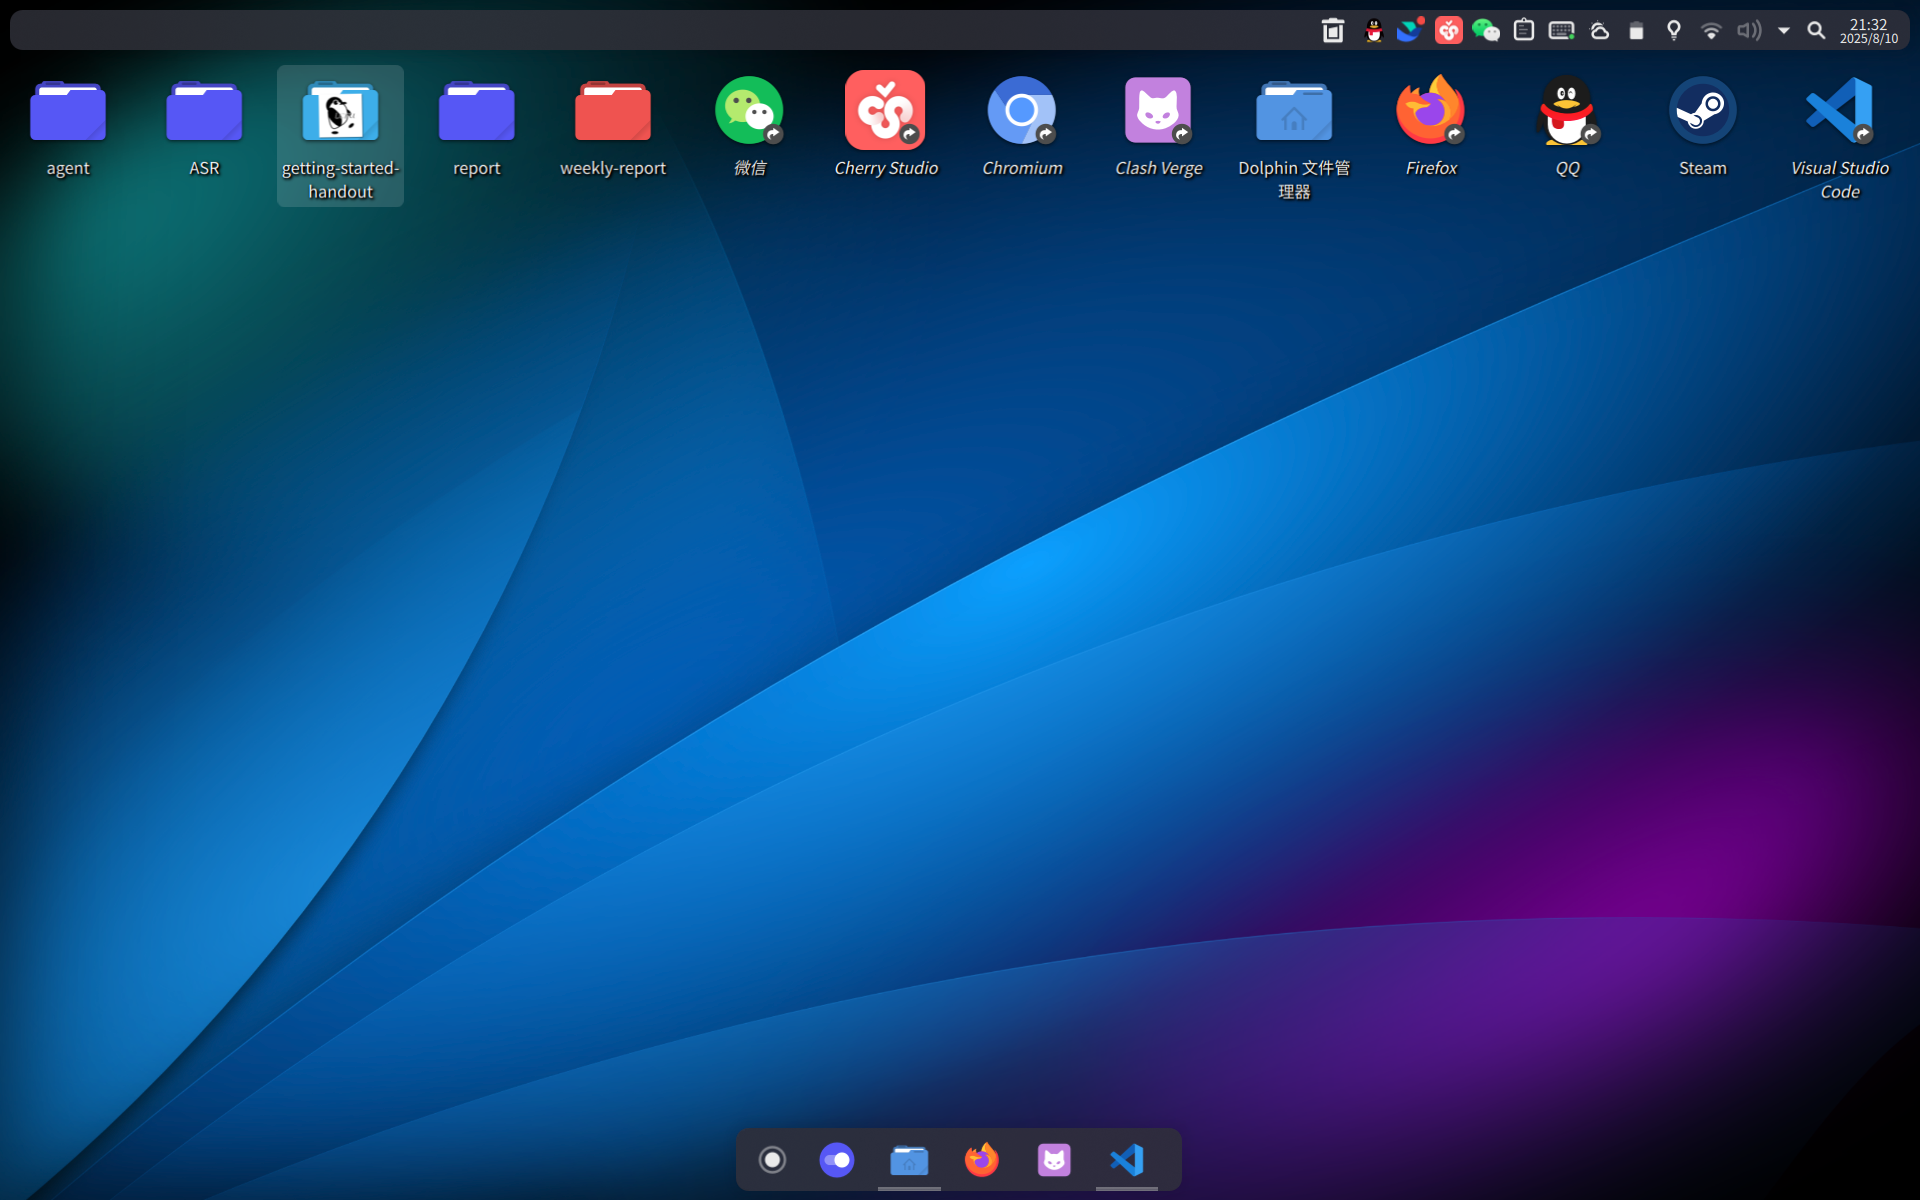
\includegraphics[width=0.8\textwidth]{100/fake-mac.png}
  \caption{一台假装自己是macOS的Arch Linux机器}
\end{figure}

\subsubsection{驱动程序}

驱动程序是操作系统和硬件之间的桥梁,它负责将操作系统的指令转换为硬件可以理解的语言。驱动程序通常由硬件制造商提供,并且在操作系统安装时自动安装。驱动程序的作用是使操作系统能够正确地识别和使用硬件设备。

驱动程序通常是特定于硬件的,因此不同的硬件设备需要不同的驱动程序。操作系统通常会自动检测硬件设备并安装相应的驱动程序,但是有时候需要手动安装驱动程序。我们可以到软件官网上下载最新的驱动程序,或者使用操作系统自带的驱动程序更新工具来更新驱动程序。不推荐使用“驱动精灵”等第三方驱动程序更新工具,因为它们可能会安装不必要的驱动程序,甚至可能会导致系统不稳定。

\subsubsection{应用软件}

应用软件指的是我们具体用于实现某一功能的工具。这类软件有很多,我们常用的通讯软件QQ、微信等,浏览网页的Chrome、Edge等,都是应用软件。

\section{计算机间的通讯}

计算机的通讯是指计算机之间或者计算机与其他设备之间进行信息交换的过程。目前计算机间的通讯主要是靠网络来实现的。网络是由许多计算机和其他设备通过通信协议连接在一起的系统,两大要素是\textbf{网络协议}(数据要依赖统一的协议传输)和\textbf{网络设备}(用于连接的设备)。

\subsection{网络基本名词及其解释}

不论是修电脑,还是平常使用计算机联网工作,我们总会在一些场合听到一些网络名词,这些网络名词不乏有被误解的。下面我们将对一些常见的网络名词进行解释。

\subsubsection{带宽、传输速率、延迟和丢包率}

这四个名词用来衡量网络的性能,是日常生活中最常见的几个名词。

\textbf{带宽}指的是网络的理论最大传输能力,通常以比特每秒(bps)或字节每秒(B/s)来衡量。带宽越大,网络的传输能力就越强。例如,一个带宽为100Mbps的网络\textbf{理论上}可以每秒传输100兆比特的数据(实际可能远低于这个数值)。我们家里通网的时候说的“千兆宽带”指的就是该网络的带宽是1000Mbps=1Gbps,或125MB/s。

而传输速率、延迟、丢包率则用于衡量网络的实际表现。\textbf{传输速率}指的是网络的实际传输速率,单位也是比特每秒(bps)或字节每秒(B/s),往往显著低于带宽。例如,一个带宽为100Mbps的网络可能实际传输速率只有50Mbps或更低。\textbf{延迟}指的是数据从发送方到接收方所需的时间,通常以毫秒(ms)为单位来衡量。延迟越低,网络的响应速度就越快。例如,一个延迟为50ms的网络意味着数据从发送方到接收方需要50毫秒的时间。\textbf{丢包率}指的是在数据传输过程中丢失的数据包的比例,通常以百分比(\%)来衡量。丢包率越低,网络的可靠性就越高。例如,一个丢包率为1\%的网络意味着在每100个数据包中有1个数据包会丢失。延迟、丢包率、传输速率等指标往往会受到网络拥塞、信号干扰、硬件性能等因素的影响。

\begin{example}
  有一辆满载硬盘的卡车从北京开到上海,估计其平均传输速率、延迟和丢包率,并和现在家用网络进行对比。
\end{example}

\begin{answer}
  先估算带宽。国内高速允许最大总重量为49吨(半挂或板车),一辆半挂车空车质量在16吨以上,这里为了方便按19吨计算,因此装载了30吨的硬盘。一块企业级数据盘容量按30TB($3\times 10^{13}$ B)计算,自重约700克;算上保护盒等,按1kg计算,因此一辆卡车装了$3\times 10^4$块硬盘,总容量为$9\times 10^{17}$ B,或者0.9EB。

  卡车在高速公路上最大时速在100到90千米每小时不等。按90千米每小时计算,北京到上海约1200千米,则行驶时间大概13.3小时,即$4.8\times 10^4$秒,因此传输速率用总数据量除以时间,得到约$1.9\times 10^{13}$B/s,即19TB/s,约合\textbf{152Tbps}。该数字非常惊人,是目前家用网络的近两万倍。

  下面估计延迟。和常规网络按数据包发送的方式不同,卡车运输是整体运输,或者说卡车本身就是一个大“数据包”,因此延迟等于运输时间,也就是从北京到上海的时间,约13.3小时,即\textbf{$4.8\times 10^4$秒}。

  下面估计丢包率。只要这个车没出事故、没被劫持、没整个掉沟里,那么就可以用公路运输HDD货物损失率0.02\%到0.05\%来充当丢包率。另外,如果出事故,则丢包率为100\%,而按照中国相关统计数据,公路运输百万公里事故数约为1起,因此完全可以忽略不计。综上,\textbf{丢包率约为0.05\%}。

  相对的,现在家用网络的传输速率大概在100MB/s到1GB/s之间,延迟大概在10ms到100ms之间,丢包率大概在0.1\%到1\%之间。可以看到,卡车运输的传输速率远远高于家用网络、丢包率显著低于家用网络,能和最优质的光纤媲美,但是延迟则高得离谱,完全无法进行实时操作。另外,卡车运输还受天气、交通等因素影响,稳定性无法和网络传输相提并论。
\end{answer}

在以往的计算机教材中总是出现一句话:“永远不要小看一辆满载磁带的卡车,其带宽远远超过了家庭网络。”看起来现在也差不多,只不过是把磁带换成了硬盘罢了;实际上,即使是2025年,把1EB数据从北京运到上海这个任务,最经济、最快速的方案依然是物流,其速度甚至能把5GB/s的高端光纤专线按在地上摩擦,成本更是低得多;只要不是那么要求时效性,物流依然是传输超大量数据的首选方案。

上述例子也提示我们怎么选择数据传输方式:GB级别的数据,可以使用任意网络途径传输;TB级别的数据,考虑使用专业的数据传输服务;PB级别的数据,考虑走光纤专线;EB级别的数据,则应考虑物流途径。要是数据量更大,那比起你把数据运过去,不如让对面把计算任务运过来。当然,上述数据是对于企业级别的网络而言的,个人用户的网络情况往往更极端,TB级别数据就可以考虑走快递等物流途径了;例如想把某些大文件从大连运送到沈阳,走网络可能需要几天时间才能传输完,而自行开车一天就能送到。

\subsubsection{IP地址和端口号}
IP地址是计算机在网络中的唯一标识符,类似于“门牌号”。目前有两种通行的IP地址:IPv4和IPv6。IPv4地址是一个32位的二进制数,通常用点分十进制数表示(例如192.168.1.1)。IPv6地址是一个128位的二进制数,通常用冒分十六进制数表示。IPv6地址的引入是为了应对IPv4地址耗尽的问题。

端口号是计算机在网络中用于区分不同应用程序的标识符,类似于“房间号”。端口号是一个16位的整数,范围从0到65535。常见的端口号有80(HTTP)、443(HTTPS)、22(SSH)等。我们假设要指向某一个计算机上的某一个应用程序,那么我们需要指定该计算机的IP地址和端口号。IP地址和端口号一起构成了一个完整的网络地址,通常表示为“IP地址:端口号”(例如0.0.0.0:8000)。

\subsubsection{域名}
域名是计算机在网络中的人类可读的标识符,类似于“网站名称”。域名由多个部分组成,通常用点分隔(例如www.pku.edu.cn)。域名系统(DNS)将域名转换为IP地址,以便计算机可以通过IP地址进行通信。

\subsubsection{子网掩码、网关}

子网掩码是一个32位的二进制数,用于划分IP地址的网络部分和主机部分。它通常用点分十进制数表示,它与IP地址进行按位与运算后,可以得到网络地址。子网掩码的作用是将一个大的网络划分为多个小的子网,以提高网络的效率和安全性。

网关是计算机在网络中的出口,用于连接不同的网络。网关通常是一个路由器或者交换机等设备。

\subsubsection{内网和外网}

我们在日常生活中,常常会听到“内网”和“外网”这两个词。内网是指一个局域网内部的网络,通常用于家庭、学校或者公司等小范围的网络。内网中的计算机可以通过路由器或者交换机等设备连接到外网。外网是指互联网上的网络,通常用于连接不同的局域网和广域网。

内网和外网的IP地址往往是不同的。内网IP地址通常是私有的IP地址,仅在内网中有效(例如每一个地级市都可能有一个“二中”,但是在不同的市称呼“二中”指的不是同一个学校);而外网IP地址全球唯一,互联网可以访问(例如“东港二中”)。例如大名鼎鼎的\texttt{8.8.8.8}是Google的公共DNS服务器的IP地址,它是一个外网IP地址。如果在内网中访问该地址,则可能访问到的不是Google的DNS服务器,而是内网中的某个设备。

\subsubsection{MAC地址}

MAC地址是计算机网络接口的唯一标识符,类似于“身份证号码”。它是一个48位的二进制数,通常用冒分十六进制数表示(例如00:1A:2B:3C:4D:5E)。MAC地址用于在局域网中唯一标识一个设备。每个网络接口卡(NIC)都有一个唯一的MAC地址。MAC地址通常由设备制造商分配,并且在设备的硬件中存储。

\subsubsection{网络协议}

网络协议是计算机之间进行通信的规则和约定。它定义了计算机如何发送和接收数据,以及如何处理错误和异常等情况。常见的网络协议有TCP/IP、HTTP、FTP等。不同的网络协议适用于不同的应用场景,例如TCP/IP协议适用于可靠的数据传输,而HTTP/HTTPS协议适用于Web应用程序的通信、UDP适用于精度要求不太高的实时通信等。

\subsubsection{网络设备}

网络设备是用于连接计算机和其他设备的硬件设备。常见的网络设备有路由器、交换机、集线器等。\textbf{路由器}用于连接不同的网络,并且可以根据网络协议进行数据转发;\textbf{交换机}用于在同一局域网内连接多个设备,并且可以根据MAC地址进行数据转发;\textbf{集线器}用于将多个设备连接到同一个网络,但不具备智能转发功能。

\textbf{光网络单元}(光猫,ONU)是用于将数字信号转换为光信号的设备,通常用于连接到光纤。光猫可以将计算机发送的数据转换为模拟信号,并且将接收到的模拟信号转换为数字信号。家用的光纤宽带通常是通过光猫连接到互联网的。

目前家用的路由器往往集成了光猫和交换机的部分功能,因此我们往往不需要像以前一样购买一大堆设备了。

\subsection{校内网络配置指南}

\subsubsection{计算机如何联网}

数据通过网络的传输需要以“数据包”的形式进行。数据包是网络传输的基本单位,它包含了发送方和接收方的IP地址、端口号、数据等信息。数据包通过网络设备(如路由器、交换机等)进行转发,最终到达接收方。

一台具体的机器,进行联网的步骤如下:
\begin{enumerate}
  \item \textbf{物理连接}:使用有线或者无线的方式,将计算机连接到网络设备(如路由器、交换机等)。
  \item \textbf{IP地址分配}:计算机通过DHCP协议自动获取IP地址、子网掩码、网关和DNS等信息。
  \item \textbf{网络协议配置}:计算机根据网络协议栈(如TCP/IP)配置网络协议,确保数据包的正确传输。
  \item \textbf{应用层协议}:计算机通过应用层协议(如HTTP、FTP等)与其他设备进行通信。
  \item \textbf{数据传输}:计算机通过网络设备和协议,将数据包发送到目标设备,并接收返回的数据包。
\end{enumerate}

\subsubsection{有线连接PKU校园网}

我们可以通过有线连接PKU校园网的方式来联网。在宿舍或者有网线接口的地方,我们可以将网线插入计算机的接口,这样就可以直接连接到校园网和互联网。

校园网的网络安全比较一般,建议购买一个路由器,连接到网线接口上,然后通过路由器连接到计算机。这样可以提高网络的安全性和稳定性。

\subsubsection{无线连接PKU校园网}

你可以在支持无线网络的设备WLAN列表中找到以下和北京大学有关的无线网络:
\begin{itemize}
  \item PKU :不安全,不建议使用。
  \item PKU Secure:采用IEEE 802.1x技术,能为用户提供较为安全的加密链路连接,一般情况下建议使用这个网络。
  \item PKU Visitor:访客网络,学生不需要使用这个。
  \item My BJMU:北大医学部的无线网络。
  \item eduroam:全球教育科研网络,该网络可以在全球许多高校使用。
\end{itemize}
具体怎样连接PKU Secure网络,请参考\href{https://its.pku.edu.cn/setting_6.jsp}{PKU Secure连接指南};使用eduroam的同学也可以参考\href{https://its.pku.edu.cn/service_1_eduroam.jsp}{eduroam连接指南}。

\subsubsection{校外连接北大内网}

为方便北京大学校园网用户在校外(家中、出差或国外)访问校园网资源,计算中心提供了VPN服务,可安全地接入校园网,如同在校内一样方便地访问学校全部的内网资源与服务(如校内门户、电子期刊数据资源等)。

具体怎样操作是一件比较复杂的事情,建议参考\href{https://its.pku.edu.cn/service_1_vpn.jsp}{北京大学VPN}的指南进行操作。

\subsubsection{北大网盘}

北大网盘是北京大学为师生提供的云存储服务,用户可以通过北大网盘存储、共享和管理文件。北大网盘提供了大容量的存储空间,并支持多种文件格式的上传和下载。

具体的使用可以参照\href{https://its.pku.edu.cn/service_1_webdisk.jsp}{北大网盘指南}进行操作。

\subsubsection{PKU腾讯会议教育版}

为了解决腾讯会议教育版资源紧张、预约繁琐的问题,计算中心上线了“腾讯会议预约申请”系统。

具体使用可以参照\href{https://its.pku.edu.cn/service_1_webex.jsp}{腾讯会议教育版指南}进行操作。

\begin{warning}
  腾讯会议教育版只用于学习和工作用途,临时、小规模或其他用途的会议请使用个人账号。
\end{warning}

\subsubsection{北大邮箱及其在第三方客户端的配置(以OutLook为例)}

北京大学为每一个新生都提供了一个北大邮箱。新生的邮箱服务一般由网易提供,地址是\texttt{<学号>@stu.pku.edu.cn}。学校的部分重要通知会发送到该邮箱上,请同学们注意查收。

方便起见,我们往往习惯于将邮箱配置到第三方客户端(如Outlook、Thunderbird等)上,以便于管理和使用。我将以Outlook为例,介绍如何配置北大邮箱。

首先,打开Outlook,点击“文件”菜单,然后选择“添加账户”。在弹出的窗口中,选择“手动进行配置”。下文使用IMAP-SMTP协议进行配置。

\begin{table}[ht]
  \centering
  \begin{tabular}{c|c|c}
    \hline
    & \texttt{pku.edu.cn} & \texttt{stu.pku.edu.cn} \\
    \hline
    IMAP服务器 & \texttt{imap.pku.edu.cn} & \texttt{imaphz.qiye.163.com} \\
    IMAP端口 & 993 & 993 \\
    \hline
    SMTP服务器 & \texttt{smtp.pku.edu.cn} & \texttt{smtphz.qiye.163.com} \\
    SMTP端口 & 465 & 994 \\
    \hline
  \end{tabular}
\end{table}

在进行正确的配置之后,Outlook会自动连接到北大邮箱服务器,此时会提示你输入用户名和密码。用户名一般是你的邮箱地址,密码则是来自特定客户端的授权码。对pku.edu.cn用户而言,授权码需在北大邮箱中获取,详见\href{https://its.pku.edu.cn/announce/tz20250702100126.jsp}{通知原文};对stu.pku.edu.cn用户而言,密码应在网易邮箱客户端中获取(登录网易邮箱网页客户端后,\texttt{设置>客户端设置>客户端授权密码})。输入正确的用户名和密码后,Outlook会自动连接到北大邮箱服务器,并开始同步邮件。

\section{网安相关知识} % Section Over

\subsection{网络的风险}

虽然互联网的出现给我们带来了便利,但也带来了很多风险。部分人心术不正,使用互联网进行诈骗、盗窃、敲诈勒索等违法犯罪活动;而他们使用的主要手段是不定向的网络攻击,例如钓鱼、木马和病毒等。

钓鱼指的是使用伪造的网页、邮件等方式,诱骗用户输入个人信息,例如用户名、密码、银行卡号等。其目的通常是获取用户的私人信息,以方便对其进行后续的诈骗、勒索等活动。

木马这个词来源于神话中的“特洛伊木马”,原指在一只巨大的木马中藏匿士兵,诱骗敌人打开城门进而发动攻击。现在的木马指一种恶意软件,它伪装成合法的软件或者捆绑在合法软件中,诱骗用户安装。一旦安装,木马就可以在用户不知情的情况下,窃取用户的个人信息、打开端口等。例如,一种最古老且经典的木马是FTP木马,它会在用户的计算机上打开一个FTP端口,允许攻击者远程访问用户的计算机。

蠕虫指的是一种自我复制的恶意软件,它可以在计算机之间传播。蠕虫通常利用计算机系统的漏洞进行传播,一旦感染了一个计算机,就会自动复制自己并传播到其他计算机。蠕虫通常会消耗计算机的资源,导致计算机变得缓慢或者崩溃。一个很经典的蠕虫是“小邮差”,它通过发送带毒邮件进行传播,会占满计算机的网络带宽;一旦感染了计算机,就会自动发送带毒邮件给其他计算机。

病毒指的是一种恶意软件,它可以在计算机之间传播。病毒通常依附在合法的软件中进行传播。病毒通常会破坏计算机的文件、数据等,导致计算机无法正常工作。一个很经典的病毒是“CIH”,它会在每年的4月26日感染计算机,并破坏计算机上的所有文件。它与蠕虫的区别是,病毒不能自己传播,只能依附于其他软件传播;而蠕虫可以自我复制。

被上述恶意软件感染后,计算机会变得不稳定、产生额外的资源开销,甚至导致计算机崩溃、数据破坏,造成经济或其他损失。君子爱财取之有道,我们应该遵纪守法,不要为了炫耀技术或者获取经济利益而制作这些恶意软件。

\subsection{从根源断绝问题}

为了防止计算机受到感染和破坏,最简单的方式是从根源上解决问题。我们在日常使用网络的时候,应该遵循以下原则:

\textbf{不浏览不安全网页}:在浏览网页的时候,若不能确定安全性,则尽量避免浏览不明链接、下载不明文件;如果确实需要下载软件,应该到官方网站上下载。

\textbf{识别伪造网站}:当一个网站需要你输入个人信息时,应该仔细检查该网站的安全性;钓鱼网站通常会伪装成合法网站,例如使用HTTPS协议、与合法网站相似的域名等。我们可以通过查看浏览器地址栏中的锁图标、检查网站的证书、观察域名是否正确等方式来判断网站的安全性。北京大学计算中心每年都会主动制作钓鱼网站,测试本校教职工和学生抗钓鱼的能力。虽然被计算中心骗了是一件不太光彩的事情,也总比被其他人骗了好,至少不会损失钱财。

\textbf{保持系统和软件的更新}:系统和软件的更新有一大部分是安全更新。定期更新软件可以阻止恶意软件利用漏洞进行攻击。

\textbf{保持杀毒软件的自动检测功能开启}:这类检测功能可以帮助我们初步检测计算机上的恶意软件。虽然有时候存在令人诟病的误报,但是它们仍然是我们保护计算机的一道重要防线。

\textbf{使用密钥代替密码}:密钥是一种更安全的身份验证方式,它可以防止密码被窃取。除了常用的公钥-私钥对,密钥还可以是USB设备、手机等。使用密钥可以防止密码被窃取和破解。目前一些技术网站已经支持使用密钥登录,例如GitHub、Google等。而我们在登录远程服务器的时候,也建议使用密钥而非密码登录。

\textbf{使用强密码并定期更换}:如果不得不使用密码登录,建议使用复杂的密码,并定期更换密码。复杂的密码应该包含字母、数字和特殊字符,并且长度至少为8位。我们也可以使用密码管理器(例如BitWarden)来生成和管理复杂的密码。

\textbf{定期备份数据}:定期备份数据可以防止数据丢失和损坏。数据备份有一个321原则:3份数据,2种介质,1个异地备份。也就是说,我们应该至少有3份数据备份,其中2份存储在不同的介质上(例如移动硬盘和云存储),1份存储在异地(例如云存储)。这样,即使我们的数据损坏了,也可以迅速恢复来减少损失。

\textbf{善用沙箱}:沙箱是一种虚拟化技术,可以将应用程序隔离在一个独立的环境中运行。这样可以一定程度上防止恶意软件对计算机造成损害。我们可以使用虚拟机、Docker等工具来创建沙箱环境,对于不能确定安全性的程序可以在此类环境中运行。

\subsection{亡羊补牢,为时未晚}

如果发现自己被钓鱼,应该紧急冻结相关账户并迅速更改密码,防止进一步的经济损失。在接下来的一个月到数个月中务必慎之又慎,你的信息可能已经被泄露,招致电信诈骗的概率显著增高。

如果发现自己的计算机感染了木马、病毒、蠕虫等,此事比被钓鱼更加严重。你应该依次执行以下内容:

\begin{itemize}
  \item \textbf{立即结束进程}:如果你能定位具体是哪一个软件正在搞破坏,可以使用任务管理器结束该进程。不过大多数情况下我们无法确定具体是哪一个进程出问题,此时忽略这一步即可。
  \item \textbf{立即断网}:这是一种负责任的行为,可以防止病毒进一步扩散。仅在软件层面上切断网络并不足够,如果你的计算机使用有线网络应该拔掉网线,以防止恶意进程重新连接网络。
  \item \textbf{立即查杀}:你可以运行杀毒软件的查杀功能,如是旧种类的病毒,杀毒软件应对起来不会太难。
  \item \textbf{立即上报}:如果杀毒软件查杀失败,应该立即上报相关部门。这可能意味着新型病毒的出现,上报有关部门有利于他们做出迅速反应,可以减少损失。
  \item \textbf{立即重装系统}:彻底重新格式化硬盘并重装系统可以彻底地清除残留的病毒文件。这是没有办法的办法,但却是最有效的。
\end{itemize}

\section{简单的计算机理论知识}

\subsection{计算机如何启动?}

我们从商店买来一台计算机,插上电源,按下电源键,计算机就启动了。这个过程发生了什么呢?硬件在这段时间内如何协同工作,使得计算机能够启动?为什么新买的计算机启动很快,而旧计算机启动很慢?为什么在更换一个性能更好的显卡之后,计算机反而启动变慢了?为了回答这些问题,我们需要了解计算机的启动过程。

计算机的启动过程可以分为以下几个步骤。

\subsubsection{加电自检}

实际上一个很反直觉的事情是,计算机在关机的时候也是一直需要通电的。计算机的主板上有一个小电池,叫做CMOS电池,它负责为计算机提供基本的电源;主板上还有一个芯片,叫做BIOS/UEFI芯片,它记录了当前时间、日期、硬件配置等信息。

当我们按下电源键时,主板收到“按下电源键”这个信号后,给电源发信号。于是电源率先启动,但它并不是立即给所有硬件供电,而是按严格的时间顺序先输出3.3V、5V、12V等不同的电压,自己也会不断检测这些电压是否在允许的误差值内。如果一切良好,电源会向主板发送一个“Power Good”信号,表示电源已经稳定工作。否则,主板会立即切断电源,防止其他硬件因错误的工作电压而损坏。

收到“Power Good”信号后,主板上的芯片组就会开始工作。芯片组会首先复位CPU,然后CPU从固定的地址开始执行整个计算机启动中的第一个指令,运行第一个程序——BIOS/UEFI程序,开始加电自检(POST,Power-On Self Test)。加电自检的任务是检测计算机的硬件是否正常工作,一般先按顺序检查CPU、内存、显卡,再检查其余设备。如果发现任何问题,加电自检会发出错误信号,例如蜂鸣声、错误代码等,提示用户进行修复。如果一切正常,加电自检会将控制权交给下一个程序。

\subsubsection{硬件初始化和配置}

POST通过后,BIOS/UEFI就会开始初始化硬件。它会为每一个PCIe\footnote{PCIe,全称Peripheral Component Interconnect Express,外设组件互连快速通道,是一种高速串行计算机扩展总线标准,用于连接主板和各种硬件设备,例如显卡、网卡、存储设备等。}设备分配总线编号、内存映射I/O空间和中断号,确保这些设备都能被操作系统正确识别。在这个时候,主板上的RGB灯、风扇、CPU超频等用户自定义配置也会被加载。

这一阶段的速度主要取决于主板固件的优化程度以及硬件的数量和类型。高端主板通常会有更好的固件优化,因此启动速度更快;而安装了大量硬件设备的计算机则需要更多时间来初始化这些设备,导致启动速度变慢。

\subsubsection{引导}

硬件准备就绪后,BIOS/UEFI就会开始引导操作系统。它会按照预设的引导顺序,依次检查硬盘、SSD、U盘、光驱等设备,寻找操作系统。传统的引导方式Legacy会读取硬盘首个扇区(MBR,512字节),该山区存放着一段大小为446字节的引导代码;而现代的UEFI引导方式则会读取EFI系统分区中的引导文件(通常是\texttt{bootx64.efi}),该文件可以存放在FAT32格式的分区中。

如果找遍整个引导顺序都没有找到操作系统,BIOS/UEFI就会发出错误信号“No bootable device”,随即终止启动过程。如果找到了操作系统,BIOS/UEFI就会将控制权交给引导加载程序(Boot Loader),开始加载操作系统。

引导加载程序又会做两件事:第一,把操作系统内核(如\texttt{winload.efi}、\texttt{vmlinuz}等)加载到内存中;第二,把启动参数(如启动分区、内核参数等)传递给操作系统内核。引导加载程序的速度主要取决于存储设备的读写速度以及引导加载程序的优化程度。

\subsubsection{内核加载与驱动初始化}

操作系统内核获得控制权后,会首先初始化CPU调度子系统、内存管理子系统,然后加载硬件抽象层(HAL)和必要的驱动程序。现在屏幕大概率会出现操作系统的Logo或者启动动画。随后,内核会并行地初始化其他设备,速度主要决定于磁盘性能、驱动数量、安全策略等因素。

\subsubsection{用户空间启动与登录界面}

现在内核初始化完毕了,可以启动第一个用户态\footnote{用户态(User Space)是指操作系统中运行应用程序的环境,与内核态(Kernel Space)相对应。用户态中的程序无法直接访问硬件资源和内核数据结构,而是通过系统调用与内核进行交互。这样可以提高系统的安全性和稳定性,防止用户程序对系统造成破坏。}进程了。在Windows中,第一个用户态进程是\texttt{smss.exe},它负责启动其他系统服务和后台进程;在Linux中,第一个用户态进程通常是\texttt{systemd}或者\texttt{init}。这些进程会负责挂载系统分区、启动日志服务、启动设备管理器等,这些都被叫做“自动启动项”。

当所有的自启动项都加载完毕,登录界面出现在屏幕上,整个启动流程结束。用户输入密码后,Explorer 或桌面环境继续加载用户级程序,至此计算机完全可用。

\subsubsection{问题解答}

现在我们就可以解答前面提出的问题了。

\textbf{为什么新旧电脑启动速度差异巨大?}

\begin{enumerate}
  \item 新主板往往用的是UEFI Fast Boot(快速启动)技术,可以跳过一些不必要的硬件检测和初始化步骤,从而大幅提升启动速度;而旧的主板往往是全部检测,耗时长;
  \item 新电脑往往使用SSD作为存储设备,SSD的读写速度和和随机读取延迟都要显著优于传统的机械硬盘,因此引导加载程序和内核加载的速度更快;
  \item 新的操作系统往往是干净的,没有太多的自启动项,因此用户空间启动的速度更快;而旧的操作系统往往安装了大量的软件和服务,导致自启动项过多,拖慢了启动速度。
\end{enumerate}

\textbf{为什么换了个高端显卡,启动反而变慢?}

实际上只有一点,也就是高端显卡的初始化时间更长。高端显卡往往有更多的功能和复杂的硬件设计,因此需要更多的时间来初始化和配置。此外,高端显卡往往需要加载更多的驱动程序和固件,这也会增加启动时间。如果主板的固件没有针对高端显卡进行优化,启动时间则会显著增加。但随着主板固件的更新和优化,这个问题会逐渐得到解决。

\begin{table}[htbp]
  \centering
  \caption{启动故障排查速查表}
  \begin{tabular}{ccc}
    \toprule
    现象 & 可能原因 \\
    \midrule
    按下电源键风扇不转 & 电源线没插、电源损坏、主板供电线松动 \\
    风扇转但没有画面 & 内存没插好、显卡供电不足、或显示器问题 \\
    主板蜂鸣器响 & 内存条松动、显卡没插好、CPU过热,具体含义见主板说明书 \\
    卡在主板Logo & 硬盘没连接好、引导顺序错误、操作系统损坏 \\
    Windows蓝屏 & 驱动程序冲突、硬件故障、系统文件损坏 \\
    Linux内核恐慌 & 硬件不兼容、驱动程序错误、文件系统损坏 \\
    \bottomrule
  \end{tabular}
\end{table}

了解启动流程后,我们就能有针对性地优化:关闭不必要的启动项、启用 Fast Boot、升级固件、更换更快的 SSD,甚至调整显卡固件设置,都能让“按下电源键到进入桌面”的时间显著缩短。

\subsection{计算机怎么和外界交互?}

我们日常把U盘插进接口,耳机塞进耳机孔,点击保存按钮把文件“放”进硬盘,仿佛计算机内部与外部世界之间隔着一堵透明的墙,数据像幽灵一样穿墙而过。实际上,这堵墙上有无数扇“暗门”,门后站着一群翻译官、调度员和安检员,它们共同把数据变成电压,把电压再变回数据,还要防止外设把奇怪的东西带进屋里。本节就拆开这堵墙,看看计算机究竟怎么和外界打交道。

\subsubsection{I/O地址和端口}

CPU 并不直接认识“鼠标”或“打印机”,它只认“地址”。x86 体系把外设抽象成一组寄存器,每个寄存器被分配一个固定或动态的 I/O 地址:早年的键盘控制器占 0x60–0x64,串口 COM1 占 0x3F8–0x3FF。CPU 用 I/O 指令像写信一样把数据塞进这些“信箱”,外设收到信后再回信,完成一次最小交互。

现代计算机中,大部分外设搬进了“内存映射 I/O”(MMIO):显卡的几百 MB 显存、NVMe 控制器的寄存器,都被映射到一段物理地址。CPU 把它们当成普通内存读写,但背后由芯片组把地址翻译成 PCIe 事务,送到目标设备。于是,同一条 mov 指令,既可能真往内存写数据,也可能改掉了显卡的光栅化参数——地址就是门牌,门牌背后是什么,由主板上的“片选信号”决定。

\subsubsection{中断与DMA}

如果CPU只能靠轮询I/O地址来和外设交互,那效率会非常低下:CPU每几毫秒就得问一次“鼠标你动没动?”,这样浪费电,速度还慢。为了解决这个问题,计算机引入了中断机制。

在外设完成动作(如鼠标拖动、键盘按键)后,它会在IRQ(中断请求线)上发出一个信号,中断控制器(现代计算机一般叫APIC,高级可编程中断控制器)收到信号后,会通知CPU暂停当前工作,转而执行一个预设的中断处理程序ISR(中断服务例程),把鼠标位移、网卡数据包什么的都统统发送,处理完毕后再返回继续执行之前的任务。这样,CPU就不需要不停地轮询外设,而是等外设主动来“敲门”,大大提高了效率。

但是中断只能通知“有事”,数据还得CPU亲自搬运,而现代SSD、千兆网卡等外设的数据量巨大,CPU搬运数据的效率远远不够。为了解决这个问题,计算机引入了DMA(直接内存访问)技术。DMA会把数据直接从外设搬到内存,CPU只需要在中断处理程序中告诉DMA控制器“把数据搬到哪里”,然后继续干自己的事。这样,CPU就能腾出更多时间处理其他任务,像稳坐钓鱼台的市长;而其他外设,如网卡、显卡、声卡等也能更高效地工作,总线就像城市立交桥一样繁忙而有序。

\subsubsection{设备驱动}

有了I/O地址、中断和DMA,CPU就能和外设打交道了。但每个外设的工作方式都不一样,CPU怎么知道该怎么和它们交流呢?这就需要设备驱动程序,它们会把数据真正翻译成外设能理解的格式,外设再把数据按人能理解的方式反馈回来。

一般情况下,设备驱动的上层会提供一个统一的抽象,下层则用无数运算把抽象翻译成具体的数据序列。驱动还要负责电源管理,例如笔记本合上盖子的时候,显卡驱动会把显存压进内存,网卡驱动会把PHY(物理层芯片)关掉,节省电量,掀开盖子再原样恢复。一个驱动bug就可能导致系统真正的“睡死过去”,因此社区经常说驱动“占了70\%的内核代码和90\%的稳定性问题”。

\subsubsection{热插拔、总线枚举}

早年的打印机必须关机才敢插拔,这叫做冷插拔。因为接口没有电气隔离,插拔时会产生电弧,烧坏接口和设备,甚至把主板烧掉。为了解决这个问题,计算机引入了热插拔技术:接口上加了电气隔离电路,插拔时不会产生电弧;操作系统也会动态识别设备的插拔事件,加载或卸载驱动程序。而其背后,是总线枚举协议在默默工作:
\begin{enumerate}
  \item 新设备插入,接口芯片检测到电压变化,向主机发“Present”信号;
  \item 主机收到信号后,在总线上广播“你是什么设备?”,设备则回复自己的ID、类型等信息;
  \item 主机根据设备信息,加载相应的驱动程序,进而分配地址、中断向量、DMA通道等资源。
\end{enumerate}

\subsubsection{从电信号到文件:以保存U盘为例}

把“保存文件到U盘”拆成时序,就能看到整条交互链:
\begin{enumerate}
\item 用户点“保存”,应用调用 \texttt{write()} 系统调用,内核把用户缓冲区映射到页缓存;
\item 文件系统(FAT32/exFAT)在缓存里分配新簇,修改 FAT 表,生成 SCSI 命令块;
\item 内核 USB 大容量存储驱动把 SCSI 命令封装成 CBW(Command Block Wrapper),交给 xHCI 主机控制器;
\item xHCI 把 CBW 切成微帧,通过差分信号线以 480 Mbps/5 Gbps/10 Gbps 速率差分发送;
\item U 盘主控收到 CBW,把逻辑块地址翻译成 NAND 物理页,拉高就绪线;
\item 主机发起 DMA,把数据突发写入 U 盘内部缓存,U 盘回传 CSW(Command Status Wrapper)表示“写完”;
\item 内核收到 CSW,把页缓存标记为干净,应用弹出“保存成功”。
\end{enumerate}
整条链路跨越用户态、内核态、USB 总线、闪存转换层,七级抽象、十几种协议,却要在几百毫秒内完成,否则用户就会抱怨“卡了”。这不禁让人感叹计算机的精密和复杂,也难怪在物流行业中计算机属于“精密仪器”或“高价值易损货物”。

\subsubsection{性能与瓶颈——为什么USB3.0跑不满5Gbps?}
\begin{itemize}
\item \textbf{协议开销:} 每 1024 字节有效数据要附带 20~30 字节包头、CRC、链路控制字,实际速率 ≈ 4 Gbps;
\item \textbf{块大小:} FAT32 默认 32 KB 簇,写小文件时主控要做“读-改-写”,带宽骤降;
\item \textbf{CPU 复制:} 若主板 USB 控制器较老,数据必须经 CPU 内存复制,吃掉 10~20\% 核心;
\item \textbf{闪存限速:} 低端 U 盘使用 TLC/QLC,持续写 1 GB 后触发缓存用尽,速度从 100 MB/s 跌到 20 MB/s。
\end{itemize}
所以,接口规格只是“天花板”,真正的地板由最慢的环节——闪存颗粒、文件系统、驱动质量——共同决定。

\subsubsection{安全关卡——I/O 权限与恶意外设}
并非所有外设都“人畜无害”。BadUSB 攻击把 U 盘固件刷成虚拟键盘,插入后自动输入恶意命令;Thunderbolt 设备通过 DMA 可直接读写整机内存,绕过 CPU 页表保护。
现代操作系统引入多层防护:
\begin{itemize}
\item \textbf{IOMMU(VT-d、AMD-Vi):} 把外设 DMA 也纳入地址转换,只允许访问内核提前登记的物理区域;
\item \textbf{代码签名:} Windows 要求内核模式驱动提交 EV 证书,无签名驱动默认拒绝加载;
\item \textbf{USB 授权弹窗:} macOS、GNOME 检测到键盘/网卡类设备首次插入时,要求用户物理点击“允许”,阻断自动注入。
\end{itemize}
即便如此,安全与便利仍像跷跷板:完全锁死外设,研究员的示波器、开发板就无法工作;全部放行,又给攻击者留下后门。操作系统每天都在这架跷跷板上找平衡。

\subsection{理解文件和目录}

文件和目录是计算机中最重要的概念之一,它们用于存储和组织计算机中的数据。

如果把硬盘看作一个图书馆,那么文件就可以看作是图书馆中的一本书。目录则可以理解为图书馆的房间、书架等,以及图书馆本身,用于组织和分类图书馆中的书籍。假如我想找到一本书,首先要知道它在哪个图书馆,其次是在哪个房间、哪个书架的哪个位置。这样就能够使用统一的方式来找到一本特定的书。

在任何计算机系统中,文件都可以看作是一些数据块。文件可以是文本文件、图片文件、音频文件、视频文件等。每一个文件都有一个唯一的名称,用于标识该文件。现代文件系统的文件名通常由字母、数字和特殊字符组成。在Windows上,文件名不区分大小写;在Linux和mac OS上,文件名区分大小写。

既然文件是一些数据块,那么就可以度量其大小。现代计算机使用二进制来表示数据,规定一个二进制位为1比特(bit),8个二进制位为1字节(Byte)。一个数据块占了多少二进制位,就可以说这个文件的大小是多少比特,或者占了比特数除以8的字节数。

在计算机上为了方便读取,之后的数据大小单位以$2^{10}=1024$为倍数递增,即1KiB=1024B,1MiB=1024KiB,1GiB=1024MiB,1TiB=1024GiB。\footnote{Windows系统中的KB指的实际上是KiB,这个是Windows本身的问题!而Linux和macOS则会正常显示KiB等。}另外一套单位系统以1000为倍数递增,也就是1KB=1000B,1MB=1000KB,1GB=1000MB,1TB=1000GB。这种标定方式便于硬件的生产,因此通常由硬件厂商使用,我们在日常生活中看到的硬盘、U盘等存储设备的容量使用的就是这种方式。因此购买的硬盘,计算机认为的容量会比标定容量小一些——这是正常现象,你的空间没有被偷窃。在TB之上还有更大的PB、EB等单位,但我们日常生活中用不到。

\begin{caution}
  有些无良卖家会使用这种单位:32Gb U盘,然后买到手发现只有4GB。这是因为该厂商使用了Gb(Gbit)而不是GB(GByte)来混淆视听,也就是32Gb=4GB,他甚至还没说谎,买家也只能打落牙齿往肚子里吞了。因此,购买存储设备时请务必注意单位究竟是什么。
\end{caution}

在Windows系统中,每一个硬盘\footnote{实际上往往是硬盘分区。在旧的计算机中,也往往叫做驱动器或卷。初学者暂时不必纠结这些概念,只需要知道有这个东西就好了。}都是一个“根”目录,相当于图书馆本身。每一个根目录都有一个盘符,例如C盘、D盘等。每一个根目录下可以有多个子目录,这些目录往往表现为文件夹的形式;每一个子目录下又可以有多个子目录,最终形成树状结构。每一个目录下可以有多个文件(相当于图书馆中的书籍)。对于一个特定的文件,从根目录到所在地的路径是唯一的,例如\texttt{C:\textbackslash Users\textbackslash username\textbackslash Documents\textbackslash file.txt}。这个完整写出来的路径叫做\textbf{绝对路径},它唯一地标识了一个文件的位置。

有时候,我们在图书馆找书的时候,知道同类的书籍往往放在一起。例如我们已经知道了这个书架上有某书第一卷,我们也知道同一个书架上还有第二卷,这时候就不需要再从图书馆的根目录开始找了,而是可以直接从这个书架上找。这时候我们可以说,第二卷的路径\textbf{相对于第一卷的路径}在同一个目录下。这个相对于某个目录的路径叫做\textbf{相对路径},它并不是唯一的,因为它依赖于当前所在的目录。举个例子,假如某文件\texttt{file1}在某目录下,同目录下还有一个\texttt{file2},那么\texttt{file2}相对于\texttt{file1}的路径就是\texttt{file2}。如果该目录下还有一个子目录\texttt{dir},该子目录下有一个\texttt{file3},那么\texttt{file3}相对于\texttt{file1}的路径就是\texttt{dir\textbackslash file3}。

有些时候,相对路径可能会跨目录,这时候就需要向上一级等操作。这时候,就可以使用“\texttt{..}”来表示上一级目录,使用“\texttt{.}”来表示当前目录。例如,假如某文件\texttt{file1}在某目录下,该目录的上一级目录下有一个\texttt{file2},那么\texttt{file2}相对于\texttt{file1}的路径就是\texttt{..\textbackslash file2}。同样,如果该目录的上级目录下还有一个子目录\texttt{dir},该子目录下有一个\texttt{file3},那么\texttt{file3}相对于\texttt{file1}的路径就是\texttt{..\textbackslash dir\textbackslash file3}。

\subsubsection{文件的扩展名}

扩展名是文件名中最后一个点后面的部分,例如\texttt{file.txt}的扩展名是\texttt{txt}。扩展名可以帮助操作系统识别文件的类型,并选择合适的程序来打开它。在Windows上,文件的扩展名往往是必须的,否则操作系统不能识别文件的类型。

在Windows系统中,文件的扩展名通常是隐藏的。如果你想查看文件的扩展名,可以在文件资源管理器中点击“查看”菜单,然后选择“文件扩展名”选项。这样就可以看到所有文件的扩展名了。为了方便维护目录等,笔者建议同学们选择显示扩展名。

\begin{table}[ht]
  \centering
  \begin{tabular}{c|l}
    \toprule
    常见文件类型 & 常见扩展名 \\
    \midrule
    文本文件 & .txt, .md, .log \\
    文档文件 & .doc(x), .xls(x), .ppt(x), .pdf \\
    图片文件 & .jpg, .jpeg, .png, .gif, .bmp, .svg \\
    音频文件 & .mp3, .wav, .flac, .aac \\
    视频文件 & .mp4, .avi, .mkv, .mov \\
    压缩文件 & .zip, .rar, .7z, .tar, .gz \\
    可执行文件 & .exe, .bat, .sh \\
    代码文件 & .c, .cpp, .py, .java, .js, .html, .css \\
    \bottomrule
  \end{tabular}
  \caption{常见文件类型及其扩展名}
  \label{tab:file-extensions}
\end{table}

一般情况下,虽然文件的类型差不多,但是其扩展名不同也往往代表着其数据的存储是按照不同的方式进行的。例如,\texttt{bmp}文件是“位图”,存储的是每一个像素的颜色信息;而\texttt{jpg}文件则是经过压缩的,存储的是图像的整体信息。对于同一张图片,\texttt{bmp}文件往往会比\texttt{jpg}文件大得多。如果我们试图将一个\texttt{bmp}文件改名为\texttt{jpg},那么这个文件的扩展名变了,但是\textbf{其内部数据并没有变},因此这个文件仍然是一个\texttt{bmp}文件,只不过扩展名变了而已。此时,如果我们使用图片查看器打开这个文件,图片查看器会根据扩展名来判断文件类型,认为它是一个\texttt{jpg}文件,但是实际上它是一个\texttt{bmp}文件,因此图片查看器可能无法正确地打开它。因此,技术人说的“一类文件”往往不是按文件的性质分类的,而是按文件的扩展名(数据的存储方式)分类的。

\subsubsection{文件的链接}

有时候,我们可能会需要在不同的目录中使用同一个文件或目录,这时候就可以使用文件的链接。文件的链接类似于图书馆中的索引卡片,它指向某个文件的位置,而不是文件本身。

上述建立链接的方式叫做软链接(符号链接)。与之相对的是硬链接,硬链接是指多个文件名指向同一个文件的数据。硬链接的创建和管理比较复杂,一般不建议初学者使用。

\subsubsection{Windows的文件系统结构}

Windows使用的是NTFS文件系统,基于驱动器(Drive),每个驱动器都有一个盘符(例如C:、D:等)。每个驱动器既可以是一个物理存储设备,也可以是一个存储设备的某一分区(主分区或者逻辑分区)。Windows的文件系统结构是树形结构,每个驱动器下都有一个根目录(例如C:\textbackslash),根目录下可以有多个子目录和文件。

在Windows下,路径使用反斜杠(\textbackslash)作为分隔符。例如\texttt{D:\textbackslash dir\textbackslash file.txt}。尽管如此,Windows也支持使用正斜杠(/)作为分隔符,两者也可以混合使用。不过我们建议在Windows下使用反斜杠(\textbackslash)作为分隔符,以保持一致性。

Windows中有如下一些常用的文件夹:
\begin{itemize}
  \item \texttt{C:\textbackslash Windows}:Windows操作系统的核心文件夹,包含系统文件和驱动程序。
  \item \texttt{C:\textbackslash Program Files}:安装的应用程序的默认文件夹,通常包含64位应用程序。
  \item \texttt{C:\textbackslash Program Files (x86)}:安装的32位应用程序的默认文件夹。
  \item \texttt{C:\textbackslash Users}:用户文件夹,包含每个用户的个人文件和设置。
  \item \texttt{C:\textbackslash Downloads}:下载文件夹,默认存储从互联网下载的文件。
\end{itemize}

\subsection{字符和编码}\label{sec:locale}

我们知道,现在的计算机是使用二进制来存储数据的。但是,对于人类使用的语言而言,即使是相对简单的英语,也有52个大小写字母、10个数字、各种标点符号和特殊符号等,远远超过了二进制的0和1两种状态;而计算机却能够正确地显示并处理这些字符。这究竟是怎么做到的呢?

一个非常容易想到的办法就是,给每一个字符分配唯一的一个编号,然后再使用二进制来表示该编号。通过建立字符和编号之间的唯一映射关系,我们就可以使用二进制来表示字符了。如果把许多个字符和编号之间的映射关系放在一起,就叫做\textbf{字符集};至于如何建立字符和编号之间的映射关系,就叫做\textbf{编码方案}。

然而,一开始,不同厂家、不同地区等生产的计算机系统使用不同的编码方案,导致同一个编码在不同的系统上表现为不同的字符,对数据交换造成了严重的障碍。我们童年时候玩的新新魔塔就是一个非常典型的例子,其标题在中国的计算机上显示为“穝穝臸娥”,其中角色“暗黑大法师”被显示为“穞堵臸猭畍”,现在这个甚至成为了一个梗。

为了解决这个问题,也容易想到两种手段:要么利用一些方法来区分不同的编码方案,并在使用时指定编码方案;要么制定一个统一的编码方案,所有的计算机系统都使用这个编码方案。然而,前者的问题非常明显:如果这么做,那么所有的计算机都要存储所有的编码方案,这非常浪费空间;而且,如果用户不知道文件使用了哪种编码方案,那么就无法正确地显示文件内容。那么制定一个统一的编码方案反而成了一个不错的选择。这或许也是新时代的“书同文”吧。

最早的统一编码方案是美国人制定的ASCII编码。该编码使用7位二进制来表示128个字符,包含了英文字母、数字、标点符号和一些控制字符。例如,字母A的ASCII编码是65,字母a的ASCII编码是97,数字0的ASCII编码是48。可是世界上并非只有英语一种语言。为了兼容法语、德语等有变音符号的语言,后来又出现了ISO-8859(以Latin-1为代表)、扩展ASCII编码等,这些编码支持更多字符。

然而,当我们把目光投向亚洲时,我们发现了新的困难:以汉语为代表的亚洲语言有着数万个甚至数十万个字符,显然超过了上述编码的范围。为了促进国际交流,世界人民最终制定了一个统一的字符集:Unicode,或“统一码”。Unicode使用16位二进制来表示65536个字符,包含了世界上所有主要语言的字符以及一些符号和表情符号,同时该编码方案也完全兼容ASCII编码和扩展ASCII编码,例如0的Unicode编码仍然是48。后来也出现了扩展Unicode编码等,可以表示更多的字符。Unicode编码的出现极大地促进了国际交流和信息共享。为了和不同的计算机相适应,Unicode编码也有多种不同的表示方式,例如UTF-8、UTF-16、UTF-32等。其中,UTF-8是最常用的表示方式,它使用1到4个字节来表示一个字符,比较节省空间。Linux和mac OS系统默认使用UTF-8编码。

如果利用错误的编码方案来读取文件,就会出现乱码的问题。以下是常见的一些乱码及其原因,我们在看到这类乱码时,可以根据其原因来判断文件使用了哪种编码方案,从而选择正确的编码方案来读取文件。

\begin{note}
  列表中“烫烫烫”等行和“锟斤拷”一同在网络上十分流行,但是和锟斤拷等不同。烫烫烫等和编码本身无关。
  
  \texttt{0xCC}等内容实际上是MSVC编译器在分配内存空间时填充的内容,\texttt{0xCC}是未分配且未赋初值的内存空间,而\texttt{0xCD}是已动态分配但未赋初值的内存空间,\texttt{0xDD}是已动态分配且已释放但未清理的内存空间。如果试图访问这些内存区域并以字符串形式打到终端上,就会出现烫烫烫等内容。

  举个有趣的例子:
  \begin{itemize}
    \item 小明煮了20个饺子。当他试图吃到第21个时,喊出“烫烫烫”。
    \item 小明说“我要煮20个饺子”但是还没煮。当他试图吃饺子的时候,喊出“屯屯屯”。
    \item 小明煮了20个饺子,吃光了并洗了碗。当他试图吃洗完的碗里的饺子时,喊出“葺葺葺”。
  \end{itemize}
\end{note}

\begin{table}[ht]
  \centering
  \caption{常见乱码以及其可能的原因}
  \begin{tabular}{c|c}
    \toprule
    乱码 & 原因 \\
    \midrule
    锟斤拷 & GBK读UTF-8 \\
    大量非法字符和西欧字符 & UTF-8读GBK \\
    仅大量西欧字符,原文变长 & Latin1读UTF-8或GBK \\
    出现大量长得像yp的东西 & UTF-8读UTF-16 \\
    大量不认识的汉字 & GBK读Big-5 \\
    \midrule
    烫烫烫 & UTF-8的\texttt{0xCC}\\
    屯屯屯 & UTF-8的\texttt{0xCD}\\
    葺葺葺 & UTF-8的\texttt{0xDD}\\
    \bottomrule
  \end{tabular}
\end{table}

由于一些历史遗留问题,在Windows系统中,如果使用中文系统,则其编码方案通常是GBK(国标扩)。然而,该编码方案并不兼容Unicode编码,因此在处理Unicode编码的文件时,可能会出现乱码的问题。为了解决这个问题,Windows系统后来也提供了Unicode编码的支持,虽然系统本身依然使用GBK编码,但是在一些应用程序中会默认使用Unicode编码,例如记事本、Word等,且这些应用程序往往会自动识别文件的编码方案并进行转换。然而,对于一些从Linux等系统中移植来的软件往往是使用Unicode而非GB2312编码的,在Windows系统中运行这些软件时,可能会出现乱码的问题,因此,我们如希望使用一些移植软件,应当避免使用中文,或者在Windows系统中使用UTF-8编码。

在Windows 10以及以后的系统中,我们可以通过\texttt{设置>时间和语言>语言>管理语言设置>更改系统区域设置},来将系统的默认编码方案更改为UTF-8编码,从而避免乱码的问题。此类编码应在系统新安装时就启用,以保证不会出现乱码问题。

\subsection{字形和字体}

刚刚我们知道了计算机中所有的字符都是通过编码来表示的。然而,电脑屏幕上的同一个汉字,往往也有着不同的表现形式。这又是怎么做到的?难不成,Unicode为同一个汉字的不同样子都分配了不同的编码?显然不是这样。实际上,Unicode只为每一个汉字分配了一个编码,而同一个汉字的不同表现形式,是通过不同的\textbf{字形}来实现的。简而言之,“字符”是它的身体,而“字形”则是它的外套。

\subsubsection{从字符到字形}

Unicode为每一个抽象字符都分配了一个唯一的编码,例如汉字“汉”的Unicode编码是U+6C49。但是这仅仅规定了这是什么字符,却并没有规定这个字符长什么样。真正的字符长相,是由\textbf{字形}来决定的。字形实际上是在计算机出现之前就已经存在的概念,指的是是字符的具体表现形式:横平竖直还是行云流水,撇是飘带还是刀刃,点是瓜子还是露珠,这些都由字形来决定。

同一个字符可以有着多种字形,这些字形可以有着不同的风格和特点。例如,宋体、黑体、楷体等都是汉字的不同字形;英语等字母语言也有不同的字形,例如Times New Roman、Arial、Courier New等。把目光放远到全世界,我们会发现同一个字符在不同的国家和地区也有着不同的字形,例如中国汉字和日本、韩国所用汉字的字形就有着明显的差异。但是它们都是同一个字符,只是字形不同而已——这便是大一统下的多样性。

\begin{figure}[htbp]
  \centering
  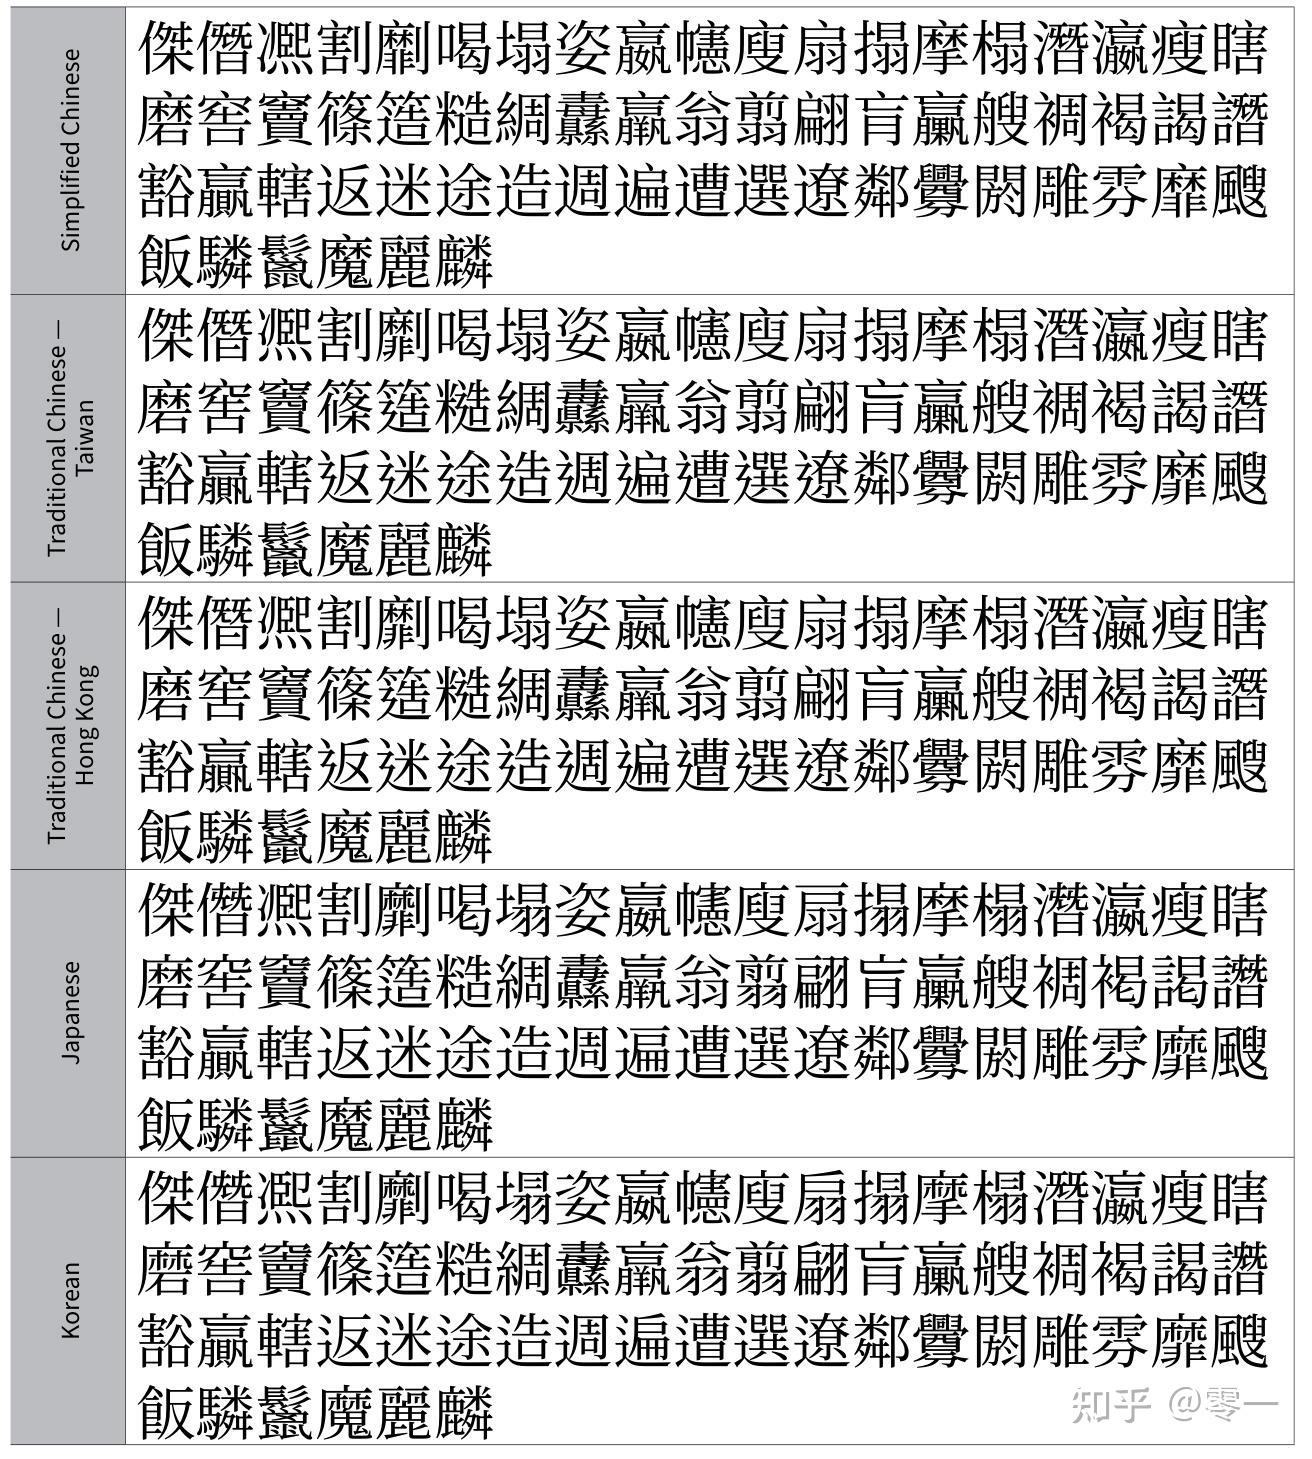
\includegraphics[width=0.5\textwidth]{100/source.jpg}
  \caption{思源字体的不同字形示例}
\end{figure}

不同的字形可以给人不同的感觉和印象,例如宋体给人正式、庄重的感觉,而楷体则给人优雅、柔和的感觉。因此,正确使用字形可以提高文本的可读性和美观性。

\subsubsection{从字形到字体}

如果把一套风格相同的字形放在一起,装进一个索引文件,再配上一个索引表,就形成了\textbf{字体文件}。当计算机试图显示一个字符的时候,它就会去字体文件中查找该字符对应的字形,然后将该字形显示出来。这个过程很容易让人想到活字印刷术:把一套字形雕刻在木块上,然后把这些木块放在一个盒子里,当需要显示某个字符的时候,就从盒子里取出对应的木块,然后将其印在纸上。而实际上一开始的确是这么做的,只是把纸张换成了屏幕罢了!

一开始,人们把字体中的每一个字形作为图片来存储,也就是所谓的“位图字体”。然而这样就会出现一个弊病:每一个字体的大小是固定的,如果我们想要一个大字体,简单地放大其图片是不行的:大家可以参考在手机上放大一张图片的效果,放大后的图片会变得模糊不清,甚至出现锯齿状的边缘。难道要为每一个字号做一个字体吗?显然不现实。

1978年,王选院士主持研制的汉字激光照排系统问世,标志着我国在汉字信息处理领域实现了从无到有的历史性突破。该系统采用了点阵字模技术,不仅可以生成不同字号的汉字,还数千倍地压缩了存储空间,极大地提高了汉字排版的效率和质量。简单地说,它突破了位图字体的局限性,正式的使得字形能够被“算出来”而不是“画出来”,这使得人们彻底打开了字体编写的思路。

1982年,Adobe推出划时代的字体格式PostScript,采用三次贝塞尔曲线来描述字形轮廓。这类字体被称为矢量字体,比王选院士的点阵字模技术更进一步。矢量字体可以通过数学公式来描述字形轮廓,因此可以任意缩放而不会失真,且文件体积较小,加载和渲染速度也较快。后来,苹果公司也推出了自己的矢量字体格式TrueType,采用二次贝塞尔曲线来描述字形轮廓,算起来更快。

之后,微软联手Adobe又搞出了OpenType字体,结合了PostScript和TrueType的优点,又能往里塞其他东西(字符变体、连字、小型大写文字、旧式数字等),成为了现在最常用的字体格式。举例说,我们现在看到的ff、fi等连字,实际上就是OpenType字体中的一个特性。汉字方面,王选院士为中文字体打下的坚实地基,也显著地促进了中文字体的不断发展。直至今日,计算机对汉字的处理方式依然是小字号点阵字模、大字号矢量字形的结合;现在,TrueType、OpenType成千上万种中文字体中数以亿计的汉字字形能够被我们随意使用,也离不开王选院士的开创性工作,王选院士也被誉为当代毕昇。

\subsubsection{从字体到屏幕}

计算机屏幕是由无数个像素点组成的,每一个像素点可以显示一种颜色。当我们试图在屏幕上显示一个字符的时候,计算机会先去字体文件中查找该字符对应的字形,然后将该字形转换为一组像素点,并将这些像素点显示在屏幕上。这个过程叫做\textbf{字体渲染}。字体渲染的过程非常复杂,涉及到许多技术和算法,例如抗锯齿、次像素渲染、字距调整等。不同的操作系统和应用程序可能会使用不同的字体渲染引擎,导致同一个字体的同一个字符在不同的系统和应用程序中显示效果不同。

\subsubsection{字重、斜体和复合字体}

在计算机出现之前,字重和斜体等就随着着印刷术的发展而出现了。字重指的是字体的粗细程度,一般可以分为Regular(常规)、Bold(粗体)、Light(细体)等。斜体指的是字体是倾斜的,一般可以分为意大利体(也叫斜体,Italic)和倾斜体(Oblique)\footnote{意大利体指的是字形本身是倾斜的,而倾斜体指的是将常规矩形字体压扁成普通平行四边形而成的字体。}。字重和斜体可以用来强调文本中的某些部分,例如标题、关键词等,从而提高文本的可读性和美观性。

在设计字体的时候,我们自然会考虑设计不同的字重和斜体版本。然而,如果为每一个字体都设计一个不同字重的版本,而不同字重的版本有的还需要斜体,这样就会导致字体文件数量爆炸,且每一个字体文件的体积也会变得很大。为了解决这个问题,我们可以使用\textbf{复合字体}。复合字体是指将多个字重和样式的字体文件组合在一起,形成一个统一的字体文件,这样不仅便于分发,也便于管理和使用。复合字体通常会包含Regular、Bold、Italic、Bold Italic等常用的字重和样式。

然而,大多数汉字字体并没有斜体字体:这是因为汉字是方块字,斜着不好看,没有这方面的需求,因此大多数汉字字体并没有斜体版本。对于英文字体而言,斜体是非常常见的,例如Times New Roman、Arial等都有斜体版本。

那有的读者会问了:为什么在MS Office中,我们能对汉字进行倾斜操作呢?这是因为,微软对斜体的定义比较宽泛:只要是倾斜的都叫斜体,而不一定非得是斜体版本的字体。对于没有斜体版本的汉字字体,微软会通过软件算法来实现倾斜效果,形成所谓的“伪斜体”。类似的,微软的Word等软件也会对没有粗体版本的汉字字体进行加粗处理,形成所谓的“伪粗体”,例如微软宋体(宋体,SimSun)就没有粗体版本,微软会通过软件算法来实现加粗效果,形成伪粗体。而对于Times New Roman等有粗体和斜体版本的字体,微软则会直接使用对应版本的字体。所以我们会发现,Times New Roman等字体的斜体和整体比起来字形有明显的差异,而宋体汉字的斜体和整体比起来字形没有明显的差异。

\subsubsection{衬线、无衬线和等宽字体}

字体可以分为衬线字体、无衬线字体和等宽字体三种类型。

衬线字体(Serif)是指在字形的笔画末端有小装饰线条的字体,例如宋体、Times New Roman等。衬线字体通常被认为更适合用于印刷品和长篇文本,因为衬线可以引导读者的视线,提高文本的可读性。无衬线字体(Sans Serif)是指没有衬线的字体,例如黑体、Arial等。无衬线字体通常被认为更适合用于屏幕显示和短篇文本,因为无衬线字体更简洁、现代,且在低分辨率下也能保持清晰。等宽字体(Monospace)是指每一个字符占用相同宽度的字体,例如Courier New、Consolas等,也叫打字机字体。等宽字体通常被认为更适合用于编程和代码编辑,因为等宽字体可以使代码更整齐、易读,且便于对齐和排版。一般的,汉字中的宋体、仿宋、楷体等是衬线字体,而黑体、微软雅黑等是无衬线字体。对于英文字体而言,Times New Roman、Georgia等是衬线字体,而Arial、Helvetica等是无衬线字体。Consolas、Courier New等是等宽字体。

同学们或许注意到了我没有说汉字的等宽字体。事实上,我们知道,汉字是方块字,每一个字它天然就是等宽的,所以为汉字设计等宽字体没有什么意义,也就没有汉字的等宽字体。一般排版中,往往使用汉字的无衬线字体(例如黑体、微软雅黑等)来搭配英文字体的等宽字体(例如Consolas、Courier New等),以达到较好的视觉效果。

\subsection{正则表达式}\label{sec:regex}

正则表达式(Regular Expression,简称Regex或RegExp)是一种用于描述字符串模式的工具。它可以帮助我们在文本中查找、替换和提取特定的字符串。正则表达式在搜索、文本处理、数据验证等方面有着广泛的应用,合理使用也能够提高工作效率。

\subsubsection{语法概要}

正则表达式的本质是“字符串匹配”,因此包括三种元素:普通字符、元字符和量词。

\textbf{普通字符}是指字母、数字和其他非特殊字符,这些字符在正则表达式中表示它们本身,例如\texttt{a}、\texttt{1}等。

\textbf{元字符}则指的是“这个字符我不确定”,例如:
\begin{itemize}
  \item \texttt{.}:匹配除换行符以外的任意单个字符。
  \item \texttt{\textbackslash d}:匹配任意数字,等价于\texttt{[0-9]}。
  \item \texttt{\textbackslash D}:匹配任意非数字,等价于\texttt{[\^0-9]}。
  \item \texttt{\textbackslash w}:匹配任意字母、数字和下划线,等价于\texttt{[a-zA-Z0-9\_]}。
  \item \texttt{\textbackslash W}:匹配任意非字母、数字和下划线,等价于\texttt{[\^a-zA-Z0-9\_]}。
  \item \texttt{\textbackslash s}:匹配任意空白字符(空格、制表符、换行符等)。
  \item \texttt{\textbackslash S}:匹配任意非空白字符。
  \item \texttt{\^}:匹配字符串的开头。
  \item \texttt{\$}:匹配字符串的结尾。
\end{itemize}
另外,如果想要匹配一组已知字符中的一个,可以使用方括号,例如\texttt{[abc]}表示匹配字符“a”、“b”或者“c”中的一个;也可以反选,例如\texttt{[\^abc]}表示匹配除“a”、“b”、“c”以外的任意字符。为了简便起见,还可以使用短横线来表示范围,例如\texttt{[a-z]}表示匹配任意小写字母。如果想匹配字符\texttt{.}本身而不是把它当作元字符使用,可以使用反斜杠进行转义,例如\texttt{\textbackslash .}表示匹配该字符本身。

而\textbf{量词}指的是“这个字符出现多少次”,例如:
\begin{itemize}
  \item \texttt{*}:匹配前面的字符零次或多次。
  \item \texttt{+}:匹配前面的字符一次或多次。
  \item \texttt{?}:匹配前面的字符零次或一次。
  \item \texttt{\{n\}}:匹配前面的字符恰好n次。
  \item \texttt{\{n,\}}:匹配前面的字符至少n次。
  \item \texttt{\{n,m\}}:匹配前面的字符至少n次,至多m次。
\end{itemize}

以上便是正则表达式的基本语法。通过组合这些元素,我们可以构建出复杂的字符串模式,从而实现强大的文本处理功能。

\begin{example}
  我们有一个文本文件,里面包含了很多电子邮件地址。我们想要提取出所有的电子邮件地址。如何使用正则表达式实现?

  提示:电子邮件地址的格式通常是\texttt{用户名@域名},其中用户名可以包含字母、数字、点、下划线和短横线,域名可以包含字母、数字和点。
\end{example}

\begin{answer}
  把一类文本转写成正则表达式的一般步骤是:先分块,然后把每一块转写成正则表达式,最后把这些正则表达式组合在一起。这个题目便是一个很好的例子。

  我们把电子邮件地址分成三部分:用户名、@ 符号和域名。然后,我们分别为每一部分编写正则表达式。

  首先,@ 符号是最简单的,因为它本身就是一个普通字符。其正则表达式就是\texttt{@}。

  然后,我们来看用户名部分。用户名可以包含字母、数字、点、下划线和短横线,因此我们可以使用方括号来表示这些字符的集合:\texttt{[a-zA-Z0-9.\_\-]}。由于用户名至少需要一个字符,因此我们可以使用量词\texttt{+}来表示这一点:\texttt{[a-zA-Z0-9.\_\-]+}。

  域名部分类似,其正则表达式为\texttt{[a-zA-Z0-9.\-]+}。注意,域名中不允许出现下划线,因此我们没有把下划线包含在方括号中。

  最后,我们将这三部分组合在一起,得到完整的正则表达式:\texttt{[a-zA-Z0-9.\_\-]+@[a-zA-Z0-9.\-]+}。这个正则表达式可以匹配所有符合电子邮件地址格式的字符串。
\end{answer}

这便是正则表达式的基本用法。正则表达式的语法和功能虽然只有这么多,但是它的应用却非常广泛。我们可以使用正则表达式来处理各种文本数据,例如日志文件、配置文件、代码文件等。正则表达式还可以用于数据验证,例如验证电子邮件地址、电话号码、身份证号码等。网上有一些有趣的正则化习题,例如一些类似word puzzle的游戏,可以帮助我们更好地理解和掌握正则表达式。

\section{初步使用计算机}

\begin{tcolorbox}[title={作为引入的笑话}, enhanced, breakable, fontupper=\small,before upper={\setlength{\parindent}{2em}}]
  你已经死了,这里是地狱!

因为你生前总是对着一堆没品笑话哈哈大笑,所以我们决定对你实施最严厉的酷刑:

——观看什么都不会的大学生操作电脑!

他在使用 Excel,但是他不会用任何一个快捷键!哦天哪他的 Ctrl 键甚至是全新的……他连自动填充和方向键都不用!从 1 到 100 都是手打的!

他输入中文的时候只用两根食指!每输入完一个词,他都用鼠标去点候选词!他一分钟打 20 个字!

他想要居中标题,在标题前面打了一连串的空格!

他直接在百度上搜 “爱奇艺下载” ,他点进了华军软件园!他点了那个最大的 “高速下载”!他直接运行了 p2p 下载器!他没有取消任何一个勾选的捆绑程序,直接点了下一步!他的桌面上多了 4 个,不,5 个,不,6 个图标!

他的表格做好了!他直接保存到 wps 云端了!他不知道如何把这份表格发给他的导师!他点了分享按钮,给导师发了一个金山文档链接!这份表格在云端查看的时候彻底乱码了!

他正在下载破解版游戏,他得到了一个压缩包!噢他没有解压缩,直接在压缩软件里点开了 \texttt{game.exe}!游戏报错了!

他终于正确地安装了一个游戏!他把 \texttt{game.exe} 直接剪切到了桌面!点开之后又报错了!

他希望把室友电脑里的游戏拷贝到自己电脑里!他把桌面上的快捷方式直接拖到了自己的 U 盘里!插回自己电脑运行的时候又报错了!

他打开文件的方式是鼠标左键疯狂连点!他至少点了 10 次!天哪现在桌面上的弹窗都堆不下了!

他把 “\texttt{Doc1.docx}” 直接重命名成了 “实验报告”!他连后缀名都删干净了!现在他再也找不到打开这份文档的方法了!

他在微信上收到了一个文件,他需要把这个文件用邮箱发出去。噢他完全不知道该怎么操作!他在收件人这一栏输入了上司的手机号!他完全不知道如何添加附件!他也完全不知道微信文件保存到哪里了!他对着微信消息按右键复制,然后把文件名粘贴到了正文栏!

他需要下载一个视频!他在视频网页点击了 “下载”,浏览器开始下载腾讯视频客户端了!他开始安装了!他在客户端里下载了一个 .qlv 格式的文件!他直接把这个文件发给别人了!

感受痛苦吧!你甚至没法教会他们!
\end{tcolorbox}

觉得眼熟?实际上,上述操作在大学生中并不少见。为了避免你也落入这种境地,下面我们介绍一些基本的计算机使用知识。

关于MS Office等办公软件的使用,建议同学们自行学习相关的教程,笔者个人特别建议使用LaTeX来代替Word和PowerPoint,而Excel则使用Python脚本或更专业的统计软件来代替。

\subsection{管理文件和目录}

\subsubsection{更改文件的类型}

有时候,我们可能会需要更改文件的类型。从上面的例子可以看出,直接更改扩展名并不能改变文件的类型,因此我们需要使用专门的软件或者网站来帮助我们转换文件的类型。例如,我们想要将一个\texttt{bmp}文件转换为\texttt{jpg}文件,我们需要使用图片编辑软件(如Photoshop、GIMP等)或者在线转换工具来进行转换。转换后,文件的扩展名和内部数据都会发生变化,变成一个真正的\texttt{jpg}文件。

\subsubsection{文件的打开方式}

对于任何文件,我们往往需要读取其中的数据,这个文件才有意义;至于这个数据是怎么展示的则另当别论。因此,我们需要一些软件来帮助我们打开文件。

在Windows系统中,文件往往有一个默认的打开方式,这个打开方式由文件的扩展名决定。例如,\texttt{.txt}文件默认使用记事本打开,\texttt{.jpg}文件默认使用照片查看器打开。有些时候安装了一些软件后,文件的默认打开方式可能会被更改。例如,安装了某个图片编辑软件后,\texttt{.jpg}文件的默认打开方式可能会被更改为该软件。

在一些情况下,我们可能会需要临时或永久更改某一类文件或者某一个文件的打开方式。我们可以右键点击文件,然后选择“打开方式”选项,选择一个合适的软件来打开该文件,也可以选择“选择其他应用”之后寻找指定的软件。如果我们想要永久更改某一类文件的默认打开方式,只需要在“选择其他应用”菜单勾选“始终使用此应用打开\texttt{.扩展名}文件”选项即可。

值得注意的是,软件本身并不需要扩展名才能打开文件。软件打开文件时总是按照自己的方式来处理数据,因此很多时候即使扩展名是错误的或者没有扩展名,如果指定了正确的软件,软件仍然可以正确地打开文件。

\subsubsection{创建文件的快捷方式}

在Windows中,文件的链接叫做快捷方式。我们可以右键点击文件,然后选择“创建快捷方式”选项,Windows会在当前目录下创建一个指向该文件的快捷方式。我们也可以将快捷方式移动到其他目录中使用。需要注意的是,快捷方式本身并不包含文件的数据,因此如果原文件被删除或者移动,快捷方式往往无法正常工作。另一方面,即使我们对快捷方式进行任意的删除或移动,原文件仍然完好无损。

\subsubsection{文件的压缩与解压}

有时候文件占据了过大的空间,或者因为文件数量太多而不便于传输和管理,这时候我们可以使用文件压缩工具来将文件进行压缩。文件压缩工具可以将多个文件或者目录打包成一个文件,并且可以对文件进行压缩,以减少文件的大小。常见的文件压缩格式有\texttt{.zip}、\texttt{.rar}、\texttt{.7z}等。

笔者个人推荐使用\texttt{7z}压缩软件来压缩和解压文件。它是一个经典的开源软件,支持多种压缩格式,并且具有较高的压缩率。一般情况下,在我们安装了\texttt{7z}软件之后,右键点击文件或者目录,就可以看到“添加到压缩文件”选项,点击该选项即可将文件或者目录进行压缩。对于压缩文件,我们也可以右键点击,然后选择“解压到当前目录”选项,或者选择“解压到\texttt{文件名}\textbackslash”选项,将文件解压到指定的目录中。

不同的压缩参数会产生不同的效果。把固实数据大小开大则会提高压缩率\footnote{压缩率是指压缩后的文件大小与原文件大小的比值,压缩率越高,说明压缩效果越好。},但会牺牲压缩和解压的速度;勾选了分卷,则会将压缩文件分割成多个小文件,便于诸如\texttt{FAT32}等不支持大文件的文件系统存储;使用内存和CPU则显著影响了压缩的速度;不同的压缩算法则会影响压缩率和速度的平衡。一般情况下,默认参数已经足够好用了,软件本身也提供了多种预设参数供我们选择。

至于压缩成的文件格式,笔者比较推荐使用\texttt{zip}格式,其兼容性最好;如果对压缩率有较高要求,可以使用\texttt{7z}格式。不建议使用\texttt{rar}格式,因为它是一个专有格式,虽然压缩率不错,但是不够开放。

\begin{caution}
  有些软件的可执行文件和附带文件是通过压缩包分发的;有些文件也是通过压缩包传输的。在这种情况下,我们一定要先解压文件,再使用文件,而不是在压缩包中直接使用文件,这样可能会导致文件无法正常工作。
\end{caution}

\subsubsection{高效的文件管理}

从一大堆文件中快速找到我们想要的文件是一个非常重要的技能。

一个常用的手段是使用搜索功能。Windows文件资源管理器提供了搜索功能,可以帮助我们找到文件。我们可以在文件资源管理器的右上角输入关键词,文件资源管理器会自动搜索当前目录及其子目录中的文件,并显示匹配的结果。然而,文件管理器的搜索面对大量文件时效率很低。这时候,我们可以使用一些第三方的搜索工具,例如Everything、Listary等。这些工具可以快速索引计算机中的文件,并提供快速的搜索功能。它们通常比文件资源管理器的搜索功能更快、更强大。

另一个常用的手段是养成良好的存储习惯,将相关的文件放在一起,使用有意义的文件名和标签、分类等工具。Windows没有内置的标签功能,但我们可以使用一些第三方的标签工具,例如TagSpaces、FileMeta等。对于大量的文件,我们可以使用自动化脚本来帮助我们管理文件,例如使用Python脚本来批量重命名文件、移动文件等。在Windows上,一个最简单的批量处理文件的方式是使用PowerShell脚本或旧式风格的批处理脚本(.bat文件)。这些脚本可以帮助我们自动化一些重复性的任务,提高工作效率。

例如,我们希望把某目录下的许多图片都改名为“图片1.jpg”、“图片2.jpg”等等。我们可以使用以下PowerShell脚本来实现:
\begin{lstlisting}
  $i = 1
  Get-ChildItem -Path "C:\path\to\your\images" -Filter *.jpg | ForEach-Object {
      $newName = "图片$i.jpg"
      Rename-Item $_.FullName -NewName $newName
      $i++
  }
\end{lstlisting}
当然用Python也行:
\begin{lstlisting}[language=python]
  import os

  path = r"C:\path\to\your\images"
  files = [f for f in os.listdir(path) if f.endswith('.jpg')]
  for i, file in enumerate(files, start=1):
      new_name = f"图片{i}.jpg"
      os.rename(os.path.join(path, file), os.path.join(path, new_name))
\end{lstlisting}
使用这些工具可以帮助我们更高效地管理文件,避免手动操作的繁琐和错误。

\subsection{怎样安装软件}

我们下载软件的主要渠道有两种:通过官方渠道下载、通过包管理器(Winget,Homebrew,apt等)下载。这两种渠道一般认为是最安全且问题最少的。官方渠道包括软件的官方网站、操作系统提供的应用商店(Microsoft Store、App Store)等;包管理器是用于管理软件包的工具。它可以自动下载、安装、升级和卸载软件包,并且可以解决软件包之间的依赖关系。

在Linux和macOS中,包管理器是非常常用的工具。它可以帮助用户快速安装和管理软件包,避免手动下载和安装软件包的麻烦。比如我希望在Arch Linux下安装GCC,只需要执行以下命令即可:

\begin{lstlisting}[language=bash]
    sudo pacman -S gcc
\end{lstlisting}

在Windows中,包管理器的使用不普遍。虽然有一个官方的包管理器winget,但是支持的软件包较少,且无法自动管理依赖(但也基本够用);还有一些例如Chocolatey、Scoop等第三方包管理器。除此以外,使用MSYS2、Cygwin等类UNIX环境也可以从某种程度上当成包管理器使用。例如后文讲的安装GCC的过程,我们就是使用MSYS2来安装的,比下载预编译版本简单许多。

我们并不推荐在非官方渠道下载软件,这些非官方渠道往往以某某软件站、某某下载站、某某应用商店(Microsoft Store这类系统自带的除外)等形式出现。通过上述方式下载的软件可能导致使用盗版、附带流氓插件甚至木马、病毒等问题,或者遇到一些其他各种问题。

如果不使用包管理器安装软件,则从官方渠道等下载的软件往往是一个压缩包或者一个可执行文件(安装包)。对于压缩包,我们只需要解压到某个目录即可使用;对于安装包,我们需要运行安装包,然后按照提示进行安装即可。为了防止过量占用C盘空间,我们建议将软件安装到非系统盘(C盘)中,例如D盘、E盘等;有些软件在安装时可能会允许你将该软件加入到系统的PATH环境变量中,我非常建议大家这么做。

\subsection{怎样卸载软件}

我们不推荐反复装卸软件,因为这可能会导致系统不稳定或者软件残留。但是有些时候,我们认为某个软件长期内不会再需要了,且磁盘空间告急,这时我们应该考虑将其卸载。

计算机小白最喜欢做的一件事是把桌面上的快捷方式移动到回收站,这是非常错误的做法。快捷方式只是指向软件的一个链接,删除快捷方式并不会卸载软件本身。对计算机半懂不懂的人喜欢找到软件的安装目录,直接删除软件的文件夹,这也是错误的做法。因为对于许多软件而言,这样做会导致软件的注册表项和其他配置文件残留在系统中,可能会导致系统不稳定或者软件无法正常工作。

正确的做法有两种:要么使用计算机自带的“程序与功能”界面删除软件,要么使用软件自带的卸载程序(通常命名为uninstall.exe或者类似名称)。某些软件可能会在安装时提供一个卸载程序,我们可以在开始菜单或者软件的安装目录中找到它。使用这些方法可以确保软件被完全卸载,留下的残留文件也较少。如要彻底删除残留文件,可以使用一些专业的卸载工具,例如Geek等。

\subsection{北京大学正版软件}

为了保护知识产权、方便学生节约资金,北京大学购买了一系列常用软件的正版授权,方便师生使用。我们可以登录\href{https://software.pku.edu.cn/}{北京大学正版软件网站},使用自己的北大账号和密码登录,下载和安装这些软件。

\subsection{软件版权和开源协议}

虽然计算机是一个非常强大的工具,但是它也可能被滥用,造成严重的后果。因此,我们需要遵守计算机伦理、法律和合规要求,以确保我们使用计算机的行为是合法和道德的。有时候我们认为稀松平常的事情,也有可能被警告。比如说用爬虫爬取IEEE论文,可能就会被IEEE警告;或者在GitHub上上传了一些别人写的GPL代码,也有可能被GitHub报DMCA警告。因此我写了本节,以提醒同学们规避风险。

软件可以认为是“数字作品”,因此也受版权法的保护。一般软件有商业软件和开源软件两种。商业软件通常是收费的,用户需要购买许可证才能使用;而开源软件则是免费的,用户可以自由地使用、修改和分发。

商业软件一般遵循专有许可证,例如微软的Windows、Office等。这些软件的源代码是保密的,用户只能使用软件的二进制文件,也不能随意修改和分发软件。这类许可证一般被叫做Copyright。对于此类软件的盗版,即使是个人使用也面临侵权风险;如果是把它用于商业则风险更大,可能面临严厉的惩罚。

而与Copy'right'相对应的也有Copy'left',即开源许可证。开源许可证允许用户自由地使用、修改和分发软件,但是需要遵守一些规定。常见的开源许可证有GPL、MIT、Apache等。这些许可证一般要求用户在分发软件时附带原始许可证,并且在修改软件时注明修改内容。

以 GPL(GNU General Public License)为例,它是最具代表性的 Copyleft 许可证之一。GPL 的核心思想是:任何人都可以自由地使用、修改和再发布软件,但如果将修改后的版本公开发布(例如发布到网上或提供给他人使用),那么整个衍生作品也必须以 GPL 许可证发布。这意味着,基于 GPL 代码开发的软件也必须开源,从而确保“自由”能够延续下去。这种“传染性”特征使得 GPL 在开源社区中备受推崇,但也引发了一些商业公司的顾虑。

除了GPL以外,还有以下这些常见的开源许可证:
\begin{itemize}
  \item MIT:MIT许可证是一种非常宽松的开源许可证,允许用户几乎无限制地使用、修改和分发软件。唯一的要求是必须在软件中包含原始许可证和版权声明。MIT许可证非常适合那些希望最大限度地推广其软件的开发者。
  \item Apache:Apache许可证也是一种宽松的开源许可证,允许用户自由地使用、修改和分发软件。与MIT许可证类似,Apache许可证要求用户在分发软件时附带原始许可证和版权声明。此外,Apache许可证还包含了一些专利授权条款,允许用户在某些情况下使用专利技术。
  \item BSD:BSD许可证是一种宽松的开源许可证,允许用户自由地使用、修改和分发软件。与MIT许可证类似,BSD许可证要求用户在分发软件时附带原始许可证和版权声明。BSD许可证有多个版本,最常见的是3-Clause BSD和2-Clause BSD。
  \item MPL:MPL(Mozilla Public License)是一种中等宽松的开源许可证,允许用户自由地使用、修改和分发软件。与GPL不同,MPL允许用户将修改后的代码与闭源代码混合使用,但要求对修改过的文件进行开源。MPL适合那些希望在保护部分代码的同时,仍然参与开源社区的开发者。
\end{itemize}

值得一提的是,开源并不等于“没有限制”。虽然用户可以自由使用、修改和分发软件,但必须遵守相应的开源许可证条款。违反这些条款,比如未按要求附带许可证、未注明修改内容,或者将 GPL 代码用于闭源商业软件,都可能构成侵权行为,甚至引发法律诉讼。


\subsection{实用软件推荐}

在学习和工作中,我们常常需要一些实用的软件来提高效率。以下是笔者个人推荐的一些实用软件,以供同学们参考。这些软件中有些是免费的,有些是收费的,具体使用时请注意软件的授权和使用条款。同时,为了防止功能冗余,我们非常建议每类软件只安装\textbf{一个}(尤其是播放器和杀毒软件!)。

\begin{itemize}
  \item 下载器类
    \begin{itemize}
      \item Internet Download Manager(IDM):一个极为强大的收费下载软件,可以显著加速下载速度,并支持断点续传等功能。遗憾的是,它不支持磁力链接和BT下载。
      \item Free Download Manager(FDM),一个免费的下载软件,界面友好且现代,且支持磁力链接和 BT 下载。
      \item 比特彗星(BitComet):一个免费且经典的BT下载软件,支持磁力链接和BT下载。
      \item qBittorrent:免费且开源的 BT 下载软件。
      \item Motrix:一个免费且开源的下载软件,支持HTTP、FTP、磁力链接和BT下载。
      \item wget:一个老牌、免费的命令行下载工具,支持HTTP、HTTPS和FTP下载。它可以通过命令行参数来控制下载行为,适合有一定技术基础的用户使用。具体使用见\ref{sec:web-get}。
      \item Aria2:一个免费的命令行下载工具,支持HTTP、FTP、磁力链接和BT下载。它可以通过命令行参数来控制下载行为,适合有一定技术基础的用户使用。
    \end{itemize}
  \item 浏览器类
    \begin{itemize}
      \item Google Chrome:一个免费的浏览器,基于Chromium内核。
      \item Mozilla Firefox:一个免费的浏览器,基于Gecko内核。
      \item 油猴:一个浏览器扩展,可以让用户自定义网页的样式和功能。它可以通过安装脚本来实现各种功能,例如广告拦截、界面美化等。油猴支持多种浏览器,包括Chrome、Firefox等。这里推荐一个链接:\href{https://github.com/zhuozhiyongde/PKU-Art}{PKU-Art},它可以给你一个风格现代、足够好看的教学网。
    \end{itemize}
  \item 压缩与解压缩类
    \begin{itemize}
      \item 7-Zip:一个免费且强大的开源老牌压缩软件,支持多种压缩格式,包括7z、zip、rar等。它的压缩率高(7z格式压缩号称全球第一压缩率),速度快,功能强大。
      \item NanaZip:在 7-Zip 基础上提供更现代化的界面(Windows 11 风格),并增加对 ZStd、LZ4 等压缩算法的编解码支持。此外,它使用 MSIX 打包,因此可上架 Microsoft Store,且可以在 Windows 11 的默认右键菜单中直接使用,而无需打开扩展右键菜单。
    \end{itemize}
  \item 播放器类
    \begin{itemize}
      \item VLC Media Player:一个免费的开源播放器,支持众多音频和视频格式。
      \item MPV:免费且开源的播放器,支持格式众多。可以使用命令行、脚本或着色器来精细地控制播放器行为,但上手难度较高。
      \item PotPlayer:另一个免费的播放器。
    \end{itemize}
  \item 杀毒软件类(Mac和Linux因为其高安全性,通常不需要安装杀毒软件)
    \begin{itemize}
      \item Windows Defender:Windows系统自带的杀毒软件,功能强大,查杀率接近100\%,已经和老牌专业杀软(卡巴斯基、BitDefender等)不相上下,能够有效地保护常规情况下计算机免受病毒和恶意软件的侵害。但是误报率较高,可能会误报一些正常的软件为病毒。
      \item 火绒:一个免费的国产杀毒软件,误报率很低,界面友好,适合普通用户使用。然而,火绒的杀毒能力要低一些。
    \end{itemize}
  \item 其他
    \begin{itemize}
      \item Everything:一个免费的文件搜索工具,能够快速地搜索计算机上的文件。它的搜索速度极快,支持多种搜索方式,包括模糊搜索、正则表达式搜索等。
      \item Wallpaper Engine:一个收费的动态壁纸软件,能够让你的桌面变得更加美观。它支持多种动态壁纸,包括视频壁纸、动画壁纸等。
      \item Rufus:一个免费的U盘制作工具,能够将ISO镜像文件写入U盘,制作成可启动的U盘。它支持多种操作系统的ISO镜像,包括Windows、Linux等。
      \item Ventoy:一个开源的u盘启动工具,能够使多个ISO镜像共存于U盘,而不必格式化U盘,选择从其中的一个镜像启动。它能使多个镜像文件和U盘其他文件共存,是装机盘和资料盘合一的好工具。
      \item UltraISO:一个收费的光盘镜像制作工具,能够创建、编辑和转换光盘镜像文件。它支持多种光盘格式,包括ISO、BIN、CUE等。
      \item VMware/VirtualBox:两个免费的虚拟机软件,能够在计算机上创建虚拟机,运行其他操作系统,可以用于测试软件、学习操作系统等。
      \item Cherry Studio:一个LLM管理器,能够帮助你使用各种LLM来简单地创建Agent,来辅助你的开发和生活。
    \end{itemize}
\end{itemize}

\begin{tip}
对于macOS用户而言,卸载软件不需要上文叙述那么麻烦,只需要将应用程序拖到废纸篓中即可。或者也可以模仿Linux常见的卸载方式,使用包管理器(如Homebrew)来卸载软件。
\end{tip}

另外,除非有相关向下兼容的需求,否则不要使用软件的过低版本。这是因为,许多软件都在不停地更新以不停的向上兼容,并修复一些已知的漏洞和问题;而过低版本的软件往往也会逐渐的停止支持。于是,过低版本的软件往往都会面临许多问题。所以我们建议同学们使用软件的一个较新版本。
\subsection{字体的安装与管理}

在Windows系统中,字体管理器可以通过控制面板中的“字体”选项来访问。用户可以将字体文件拖放到该窗口中来安装字体,或者右键点击字体文件并选择“安装”来安装字体。卸载字体也可以通过右键点击字体文件并选择“删除”来完成。用户还可以通过该窗口来预览字体文件,并查看字体的详细信息,例如字重、样式、版本等。

\subsection{计算机的日常维护}

计算机的维护是一个非常重要的环节。我们需要定期对计算机进行清理和维护,以保证计算机的正常运行。

\subsubsection{保持更新系统的习惯}

计算机在运行过程中,操作系统和软件会不断地更新,以修复漏洞、提高性能和增加新功能。我们应该定期检查系统和软件的更新,并及时按需要安装它们。

对于一些重要的更新(例如安全更新等),我们应该立即安装,这是因为此类更新通常是为了修复一些新近发现的漏洞和问题,如果不及时安装,可能会导致计算机被攻击或者出现其他问题。而对于一些不重要的更新(例如功能更新等),我们可以根据自己的需要选择安装。

\begin{caution}
  虽然我们提倡保持更新,但是在生产类环境中,贸然更新可能会导致系统不稳定或软件不兼容。因此,在生产环境中,我们应该在更新之前进行充分的测试,确保更新不会影响系统的正常运行,或者使用虚拟机等隔离环境运行生产用代码。
\end{caution}

\subsubsection{定期备份数据}

定期备份数据是保护计算机数据安全的重要措施。我们可以使用外部硬盘、云存储等方式备份数据,以防止信息泄露或者重要文件丢失。数据备份的频率可以根据数据的重要性和变化频率来决定。

数据备份有一个重要的原则:\textbf{3-2-1备份法则}。即:至少保留三份数据备份,存储在两个不同的介质上,其中一份存储在异地。例如,我们可以在本地硬盘上存储一份数据备份,在外部硬盘上存储一份数据备份,并将另一份数据备份存储在云端。这样,即使其中一份甚至两份损坏或者丢失,我们也可以通过其他方式恢复数据。

\subsubsection{定期清理系统}

定期清理系统可以提高计算机的性能和安全性。我们可以使用一些系统清理工具,删除不必要的文件、缓存和临时文件等,以释放磁盘空间和提高系统性能。我们推荐使用系统自带的清理工具,例如Windows的磁盘清理工具、macOS的存储管理工具等。如果较为富裕,也可以使用一些知名的清理软件,例如CCleaner等(免费版已经足够好用了)。出于众所周知的原因,我们不推荐使用360等软件。

除此之外,休眠文件、系统还原点等也会占用大量磁盘空间。我们可以根据自己的需要,选择是否保留这些文件。

\begin{caution}
  清理系统和减肥差不多,同样需要\textbf{缓慢、谨慎、循序渐进}地进行,不要一口气删除大量内容,如果必要还应预先备份或者创建系统还原点等。
\end{caution}

\subsubsection{碎片整理}

在计算机使用过程中,如果使用机械硬盘,文件的删除和修改会导致磁盘上的数据变得零散,从而影响计算机的性能。我们可以使用碎片整理工具,定期对磁盘进行碎片整理(即重排文件使其连续),以部分提高磁盘的读写速度。

直接使用Windows自带的碎片整理工具即可。对于固态硬盘,碎片整理并不会提高性能,反而会缩短使用寿命,因此不建议对SSD进行碎片整理。

\subsection{善用键盘}

我们早就知道如何使用键盘了,几乎所有人都会使用键盘来进行文字输入等操作。但是键盘上还有一些较为特殊的按键,它们虽然不具体对应某一个字符,但是却能帮助我们更高效地和计算机交互。

\subsubsection{修饰键等特殊按键}

大多数键盘上都有着成对的\texttt{Ctrl}、\texttt{Alt}、\texttt{Shift}等按键,这些按键通常被称为“修饰键”。

常见的修饰键有以下几种:
\begin{itemize}
  \item \texttt{Ctrl}(Control):控制键,通常用于执行各种命令和操作。
  \item \texttt{Alt}(Alternate):替换键,通常用于切换窗口、菜单等。
  \item \texttt{Shift}:换档键,通常用于输入大写字母和特殊符号。
  \item \texttt{Win}(Windows键):Windows徽标键,通常用于打开开始菜单、切换窗口等。这个键仅在Windows系统中存在,在Linux中被叫做\texttt{Super}或\texttt{Meta}键,在macOS中被叫做\texttt{Command}键。
  \item \texttt{Fn}(Function):功能键,通常用于切换键盘的功能模式,例如调整音量、亮度等。这个键不是每一个键盘上都有。
\end{itemize}

除修饰键和字母、数字外,还有一些特殊按键。这些案件也可以帮助我们高效地和计算机交互。
\begin{itemize}
  \item \texttt{Esc}(Escape):退出键,通常用于退出当前操作或者关闭窗口等。
  \item \texttt{Tab}(Tabulator):制表键,通常用于切换输入焦点或者插入制表符等。
  \item \texttt{Caps Lock}:大写锁定键,按下后可以输入大写字母,按下再次取消。
  \item \texttt{PrtScn}(Print Screen):打印屏幕键,通常用于截取屏幕内容。在不同的计算机上也有不同的名字。
  \item \texttt{Pause Break}:暂停键,通常用于暂停程序的执行。在现代计算机上,这个键很少使用。
  \item \texttt{Scroll Lock}:滚动锁定键,通常用于锁定滚动功能。在现代计算机上,这个键很少使用。
\end{itemize}

一开始的键盘是为了和终端(黑窗口)交互的,为了操作光标,因此也有着一些光标控制键:
\begin{itemize}
  \item 方向键(上下左右箭头):用于控制光标的移动。
  \item \texttt{Home}:光标移动到行首。
  \item \texttt{End}:光标移动到行尾。
  \item \texttt{Page Up}:向上翻页。
  \item \texttt{Page Down}:向下翻页。
  \item \texttt{Delete}:删除键,通常用于删除光标后的字符,与\texttt{Backspace}正好相反,后者用于删除光标前的字符。
  \item \texttt{Insert}:插入键,通常用于切换插入模式和覆盖模式。
\end{itemize}

\subsubsection{高效打字}

虽然很多人都会打字,但是打字的效率却参差不齐。除了使用上述的修饰键和特殊按键以外,我们还可以通过一些方法来提高打字效率。

首先,实际上打字是有一个正确的姿势的。这个姿势要求两只手的食指分别放在键盘的F和J键上,这两个键被叫做“基准键”。在漫长的使用过程中,可能基准键会随着习惯而有所偏移(例如笔者的习惯是将D和H作为基准键,这样比较灵活的右手会辐射更大的范围),这并不需要纠正,因为习惯下来也没什么大问题。但是不管怎么样,最终\textbf{你十个手指当中的大多数在打字过程中要动起来},而不是二指禅,这样才能提高打字效率。

另外,打字是一个熟练工作,只有多练习才能提高打字速度和准确率。打字较快的人大多数都会盲打,也就是在打字的时候眼睛仅盯着输入法选字窗口,而不看键盘。这样可以减少眼睛在键盘和屏幕之间的移动,提高打字效率。我们推荐使用一些打字练习软件,例如TypingClub、Keybr等,来提高打字速度和准确率。

有些人会问五笔和拼音哪个打字更快。实际上,五笔的极限速度要高于拼音,对于打字员等专业人士而言,他们打字的时候眼睛只看着手写或打印的纸张,屏幕和键盘都不看;他们和抄写一样,直接复制字形并打出编码,因此五笔的速度会更快一些。但是,五笔是违反人语言习惯的输入法:我们在写东西的时候,往往是先想到词语的发音,然后再想到字形,而五笔则是直接根据字形来输入,这对于大多数人而言并不自然。因此,对于大多数人而言,拼音输入法更为合适。另外,随着技术的不断进步,现代的大多数输入法连接了网络,能够通过用户的上文推测下文大概是什么词语,从而提高了输入效率,可以媲美甚至超越五笔的极限速度。

\subsubsection{快捷键}

当我们按下这些按键时,再按下其他按键,就可以实现更多的功能。这样的按键组合就叫做“快捷键”。使用快捷键可以减少鼠标操作的频率。以下是来自Windows的常用快捷键:

\begin{table}[ht]
  \centering
  \caption{Windows常用快捷键}
  \label{tab:windows-shortcuts}
  \begin{tabular}[t]{c|c}
    \hline
    \textbf{快捷键} & \textbf{功能} \\
    \hline
    \texttt{Ctrl+C} & 复制 \\
    \texttt{Ctrl+V} & 粘贴 \\
    \texttt{Ctrl+Z} & 撤销 \\
    \texttt{Ctrl+Y} & 重做 \\
    \texttt{Ctrl+A} & 全选 \\
    \texttt{Ctrl+Alt+Del} & 打开任务管理器 \\
    \texttt{Ctrl+S} & 保存当前文档或文件 \\
    \texttt{Ctrl+P} & 打印当前文档或文件 \\
    \texttt{Ctrl+F} & 查找文本或内容 \\
    \hline
  \end{tabular}
  \qquad
  \begin{tabular}[t]{c|c}
    \hline
    \textbf{快捷键} & \textbf{功能} \\
    \hline
    \texttt{Alt+F4} & 关闭当前窗口 \\
    \texttt{Alt+Tab} & 迅速切换窗口 \\
    \texttt{Win+R} & 打开运行窗口 \\
    \texttt{Win+E} & 打开文件资源管理器 \\
    \texttt{Win+D} & 显示桌面 \\
    \texttt{Win+L} & 锁定计算机 \\
    \texttt{PrtScn} & 截图(全屏) \\
    \texttt{Alt+PrtScn} & 截图(当前窗口) \\
    \texttt{Win+Shift+S} & 截图(自定义区域) \\
    \hline
  \end{tabular}
\end{table}

除了上述快捷键以外,在其他的软件中也有着自己特定的快捷键。例如在浏览器中,\texttt{Ctrl+T}可以打开一个新的标签页,\texttt{Ctrl+W}可以关闭当前标签页,\texttt{Ctrl+Shift+T}可以重新打开上一个关闭的标签页等。这些快捷键可以帮助我们更高效地使用计算机。

\subsection{使用终端}\label{sec:terminal}

终端是计算机与操作系统之间的一个交互界面。它允许用户通过命令行输入指令,与操作系统进行交互。

虽然终端是一个非常古老的工具,但是使用它依然可以提高工作效率,尤其是在处理大量文件或者进行复杂操作时。它还可以用于远程连接到其他计算机,进行远程管理和维护等操作。

一般情况下,一条命令满足以下结构:
\begin{lstlisting}[language=bash]
    <命令> [<选项>] [<参数>]
\end{lstlisting}

其中,命令是要执行的操作,选项是对命令的补充说明(例如 -h 往往表示帮助信息),参数是命令的输入(例如文件名)。选项和参数往往都是可选的。

对于Linux和macOS,常见的shell有以下几种:

\begin{table}[ht]
  \centering
  \begin{tabular}{c|ccc}
    \toprule
    & \textbf{bash} & \textbf{zsh} & \textbf{fish} \\
    \midrule
    定位 & 通用,默认 & 高度定制 & 易用、美观、现代化 \\
    兼容性 & POSIX标准兼容 & 大多数兼容bash & 不兼容bash,自成一套 \\
    上手难度 & 中等 & 中等偏高 & 非常简单 \\
    自动补全 & 仅有基础功能 & 需配合插件 & 开箱即用 \\
    语法高亮 & 没有 & 有插件 & 默认有 \\
    可定制性 & 较低 & 非常高 & 较高 \\
    脚本通用性 & 几乎全通用 & 高 & 低 \\
    资源占用 & 非常低 & 取决于插件 & 较低 \\
    \bottomrule
  \end{tabular}
  \caption{常见的Linux/macOS Shell对比}
\end{table}
我们推荐使用zsh或者fish。关于zsh怎么安装插件的问题,可以参考网上的各种教程,例如Oh My Zsh等。

对于Windows,默认的终端是CMD,其风格太老了,基本与现代开发脱节,不建议使用。我们建议使用Windows PowerShell。PowerShell的命令统一采用的是动词-名词的格式,和Linux Shell的简单缩写形式有很大的不同。这是因为PowerShell的设计理念是模仿C\#的“对象”,而不是Linux Shell的文本流。不过也正因此,PowerShell本身就是一门完备的语言,功能非常强大,在处理复杂的任务上更为简单。

除了这些以外,如果不希望使用Windows的原生终端,也可以使用诸如Cygwin、MSYS2等类UNIX环境,来获得类似Linux的终端体验。有些教程会让你使用git bash,这东西是一个精简版MSYS2,主要用于Git操作,功能非常有限,不建议长期使用。

下表\ref{tab:terminal-commands}是一些常见的命令。

\begin{table}[ht]
  \centering
  \begin{tabular}{c|cc}
    \hline
    \textbf{操作} & \textbf{Bash等} & \textbf{Pwsh} \\
    \hline
    创建文件 & touch & New-Item \\
    列出文件 & ls & Get-ChildItem \\
    复制文件 & cp & Copy-Item \\
    移动文件 & mv & Move-Item \\
    删除文件 & rm & Remove-Item \\
    创建目录 & mkdir & New-Item -Type Directory \\
    删除目录 & rmdir & Remove-Item -Recurse \\
    查看帮助 & man & Get-Help \\
    \hline
  \end{tabular}
  \caption{Bash和PowerShell的常用命令对比}
  \label{tab:terminal-commands}
\end{table}

当然,上述命令在Windows上并不常用。我在这里提到终端的目的主要是为了让同学们了解终端的存在,并且知道它的基本用法。对于日常使用,图形界面已经足够好用了;然而,如果想从事开发,终端反而会变得不可或缺,尤其是在使用诸如Git、Docker等工具时。另外,在希望对文件进行批量处理时,终端也会显得非常有用。

例如,“Windows聚焦”每天都会更新新的图片,例如风景、动物等,并将其作为锁屏背景或桌面背景。这些图片被缓存储在一个隐藏目录中,且没有扩展名。如果遇到特别喜欢的图片,可以把这些缓存提取出来,并批量加上扩展名:
\begin{lstlisting}
  Rename-Item -Path "Your\Path\Here\*" -NewName { $_.Name + ".jpg" } # Pwsh 风格
  ren Your\Path\Here\* *.jpg # CMD 风格,一般Pwsh兼容
\end{lstlisting}
这样比起手动地一个个添加扩展名要方便得多。

\subsection{初级自动化:计划任务}

有些任务是重复性的,例如每天定时备份数据、每周定时清理系统等。对于这些任务,我们可以使用计划任务来自动化它们。Windows提供了计划任务功能,可以帮助我们定时执行某些任务。

我们可以通过以下步骤创建一个计划任务:
\begin{enumerate}
  \item 打开“任务计划程序”:可以通过开始菜单搜索“任务计划程序”来打开。
  \item 创建基本任务:在任务计划程序中,点击“创建基本任务”选项,输入任务的名称和描述。
  \item 设置触发器:选择任务的触发条件,例如每天、每周等。
  \item 设置操作:选择要执行的操作,例如启动程序、发送电子邮件等。
  \item 设置参数:输入要执行的程序的路径和参数。
  \item 完成任务创建:点击“完成”按钮,任务就创建好了。
\end{enumerate}

\subsection{正确且高效地获取网站资源}\label{sec:web-get}

在学习和工作中,我们常常需要从网站上获取一些资源,例如图片、视频、文档等。然而,在部分网站上,想直接下载这些资源并不容易。我们可以使用一些工具和方法来帮助我们获取这些资源。

\subsubsection{网站抓取}

一个最常规的方法是使用网站抓取工具,例如HTTrack、wget等。这些工具可以帮助我们下载整个网站或者部分网站的内容,并且可以设置一些选项,例如下载深度、文件类型等。wget是非常老牌的网站抓取工具,我将在这里介绍它的基本用法。

wget的基本语法如下:
\begin{lstlisting}[language=bash]
    wget [选项] [URL]
\end{lstlisting}
URL是要下载的资源的地址,选项是对下载过程的补充说明。实际上这个选项才是重头戏。以下是一些常用的选项:
\begin{itemize}
  \item \texttt{-r}:递归下载,即下载整个网站或者部分网站的内容。
  \item \texttt{-l <深度>}:设置下载的深度,例如\texttt{-l 2}表示下载两层目录。
  \item \texttt{-A <文件类型>}:设置要下载的文件类型,例如\texttt{-A jpg,png}表示只下载jpg和png格式的文件。
  \item \texttt{-P <目录>}:设置下载的目录,例如\texttt{-P /home/user/downloads}表示将下载的文件保存到指定目录。
  \item \texttt{-c}:断点续传,即如果下载过程中断,可以从中断的地方继续下载。
  \item \texttt{-e robots=off}:忽略网站的robots.txt文件,强制下载所有内容。该选项可能会违反网站的使用条款,请谨慎使用。
  \item \texttt{-q}:安静模式,不显示下载过程中的信息。
  \item \texttt{-O <文件名>}:将下载的内容保存为指定的文件名。
\end{itemize}

例如,某网页地址为\url{http://example.com/files.html},该网页上有很多文件的链接,我们想要下载所有的PDF文件,可以使用以下命令:
\begin{lstlisting}[language=bash]
  wget -r -l 1 -A pdf -P ./downloads http://example.com/files.html
\end{lstlisting}
该命令会递归下载该网页上的所有PDF文件,并将其保存到当前目录下的downloads文件夹中。

另一个简单的使用例子是下载单个的文件:
\begin{lstlisting}[language=bash]
  wget --show-progress -P ~/Downloads http://example.com/data_clip.zip
\end{lstlisting}
一般情况下我个人习惯使用\texttt{--show-progress}来显示下载进度,且不使用\texttt{-q}来隐藏下载信息,这样可以方便地查看下载的进度和状态。

wget适用于抓取网站的静态资源,例如图片、文档等。然而,现在很多网站都是动态的,例如Bilibili的播放页面的工作原理是:首先加载一个HTML页面,然后通过JavaScript代码从服务器获取视频的真实地址,在这个过程中还需要进行鉴权等操作。对于这种网站,wget这种静态抓取工具就不能使用了。对此,应使用更激进的手段,如爬虫等。也可以使用专门的下载工具(例如youtube-dl、yt-dlp、IDM的浏览器插件),这些工具可以帮助我们获取动态网站的资源。

\subsubsection{浏览器开发者模式}

现代浏览器都提供了开发者模式,可以帮助我们查看网站的源代码、网络请求等信息。我们可以通过按下\texttt{F12}键或者右键点击页面选择“检查”来打开开发者模式。在开发者模式中,我们可以查看网站的HTML代码、CSS样式、JavaScript代码等内容,还可以查看网络请求,找到资源的真实地址。另外,还可以输入一些JavaScript代码来帮助我们调试。这个功能难度比较大,建议有兴趣的同学自行学习。

\begin{thinking}
\begin{enumerate}
  \item 为什么差分机、电子管、晶体管、IC、SoC每一次换代都能带来计算机性能的显著提升和能耗十倍级下降?未来的计算机硬件会朝着什么方向发展?现在量子计算机已经有了雏形,未来会不会继续遵守这条能源曲线?
  \item 因为内存速度跟不上CPU的速度,所以出现了缓存(Cache)这种东西。如果直接把计算单元做进DRAM中会怎么样?为什么现在的计算机没有广泛使用这种设计?
  \item SSD、HDD、光盘都是常见的存储介质。上述硬件分别使用什么原理来存储数据?为什么它们的读写速度差别如此之大?使用不同介质存储冷数据和热数据,威胁存储稳定性的主要因素有哪些?
  \item Unicode统一了码表。众所周知,汉语、日语、韩语均使用或部分使用汉字(谚文),且其字形略有区别。Unicode是如何处理相同汉字的不同字形的?这对OCR、版权取证、司法勘验等领域有何影响?如果你是设计者,你会如何解决这些问题?
  \item GPL协议有传染性。但是在法律实践中,分离性边界的划分并不相同。例如,中国2021柚子案和德国2021Nextcloud案的结论恰恰相反,技术专家在该方面出具了什么意见?你能否试着总结出可量化的“传染概率”?
\end{enumerate}
\end{thinking}